
\documentclass[10pt]{article}

% !TEX root = ../master.tex

% =============================================================================
% preamble.tex --- shared package loads and formatting for the Earthquake
% Source Mechanics lecture notes. \input{} this from master.tex, after
% \documentclass and before \begin{document}.
% =============================================================================

\usepackage{graphicx}
\usepackage[a4paper,left=2cm,right=2cm, bottom=2.cm, top=2.0cm]{geometry}
\usepackage{amssymb}
\usepackage{amsmath}
\usepackage{mathtools}   % extends amsmath: needed for psmallmatrix, etc.
\usepackage{bm}
\usepackage{longtable}
\usepackage[margin=1pt,font=small,labelfont=bf]{caption}
\usepackage[dvipsnames]{xcolor}
\definecolor{citecolor}{RGB}{128,0,32}
\usepackage[unicode,hyperfootnotes=false,breaklinks=true,colorlinks=true,allcolors=blue]{hyperref}
\usepackage{setspace}
\usepackage{fancyhdr}
\usepackage{titlesec}
\usepackage{algorithm}
\usepackage{algpseudocode}
\usepackage{etoolbox}
\newcommand{\degree}{\ensuremath{^\circ}}

\usepackage{times}      % or whatever Plex text variant you want


\usepackage{tabularx}
\usepackage{booktabs}   % needed for the elastic-constants tables in lecture01
\usepackage{datetime}
\usepackage{lineno}
\usepackage{etoolbox}
\usepackage[utf8]{inputenc}   % if not already present
\usepackage[T1]{fontenc}      % this is the one that fixes your error
\usepackage[french,english]{babel}    % english is last-loaded => main/document language;
                                       % french stays available (e.g. via \foreignlanguage{french}{...})
                                       % without which \guillemetleft would misbehave, per original note
\usepackage[normalem]{ulem}  % normalem keeps \emph as italic, not underlined
\usepackage{csquotes}
\usepackage{tikz}
\usetikzlibrary{arrows.meta, angles, quotes, decorations.pathreplacing, positioning, calc, decorations.pathmorphing}
\usepackage{enumitem}
\setlist[itemize]{itemsep=0pt, topsep=2pt, parsep=0pt}

\patchcmd{\linenumber}{\hb@xt@}{\hbox}{}{}

\newdateformat{usvardate}{\shortmonthname[\THEMONTH]. \THEDAY, \THEYEAR}
\newcommand{\lastmodified}{%
  \textcolor{citecolor}{\scriptsize \usvardate\today{}}
}
\setlength{\parindent}{0pt}
\setlength{\parskip}{1em}
\renewcommand{\headrulewidth}{0.0pt}
\renewcommand{\footrulewidth}{0.0pt}
%\setlength{\headheight}{15pt}
\fancypagestyle{custom}
{
\fancyhead[L]{}
\fancyhead[C]{}
\fancyhead[R]{}
\fancyfoot[L]{\textcolor{gray}{\bf DRAFT has errors}}
\fancyfoot[C]{\textcolor{gray}{\thepage}}
%\fancyfoot[R]{\lastmodified}
\fancyfoot[R]{}
\fancyfoot[L]{}
}

\renewcommand\thesection{\arabic{section}}
\titlespacing\section{0pt}{12pt plus 4pt minus 2pt}{0pt plus 2pt minus 2pt}

%-----------------------------------------------------------------------------
% Table of contents: show \part and \section entries only (hide \subsection
% and deeper), make the spacing between entries compact, indent the
% \section entries under their \part entry, and drop the section numbers
% from the TOC listing (the numbers/\ref's in the body text are untouched --
% this only changes how entries are printed in the Contents list). The
% \parskip leaking into the TOC's own paragraphs is neutralized locally
% around the \tableofcontents call itself, in master.tex.
%-----------------------------------------------------------------------------
\setcounter{tocdepth}{1}

\makeatletter
\patchcmd{\l@part}{\addvspace{2.25em \@plus\p@}}{\addvspace{0.8em \@plus\p@}}{}{}

\renewcommand*\l@section[2]{%
  \ifnum \c@tocdepth >\z@
    \addpenalty\@secpenalty
    \addvspace{0.1em \@plus\p@}%
    \begingroup
      \renewcommand\numberline[1]{}%   % suppress the section number in the TOC
      \parindent \z@ \leftskip 1.5em \rightskip \@pnumwidth
      \parfillskip -\@pnumwidth
      \leavevmode \small
      #1\nobreak\hfil \nobreak\hb@xt@\@pnumwidth{\hss #2}\par
    \endgroup
  \fi}
\makeatother
%-----------------------------------------------------------------------------
% Bibliography management
%-----------------------------------------------------------------------------
% JGR style citations
\usepackage[
  giveninits=true,
  style=authoryear,
  backend=bibtex,
  maxcitenames=2,
  maxbibnames=99,
  hyperref=true,
  backref=false,
  sorting=nyt,
  uniquename=init,
  autolang=hyphen,
  dashed=false]{biblatex}

\AtEveryCite{\it \color{citecolor}}
\AtEveryBibitem{\clearfield{month}}
\setcounter{biburlnumpenalty}{100}
\setcounter{biburlucpenalty}{100}
\setcounter{biburllcpenalty}{100}
\renewcommand*{\finalnamedelim}{\addspace\&\space}
\AtEveryBibitem{\clearfield{issn}}
\renewbibmacro{in:}{}
\AtBeginDocument{%
  \renewcommand*{\mkbibnamefamily}[1]{#1}%
  \renewcommand*{\mkbibnamegiven}[1]{#1}%
  \renewcommand*{\mkbibnameprefix}[1]{#1}%
}

\definecolor{darkgreen}{rgb}{0.15,0.55,0.35}
\newcommand{\todo}[1]{\textcolor{darkgreen}{\textbf{[TODO: \uline{#1}]}}}
\newenvironment{itemize*}%
  {\begin{itemize}%
    \setlength{\itemsep}{0pt}%
    \setlength{\parskip}{0pt}}%
  {\end{itemize}}

%\linenumbers
%-----------------------------------------------------------------------------
% Line spacing
\setstretch{1.05}
%-----------------------------------------------------------------------------
% Graphics and bibliography paths
%-----------------------------------------------------------------------------
\graphicspath{{./lectures/figures/}}
\addbibresource{./lectures/MasterBibliography.bib}

% =============================================================================
% symbols.tex --- custom macros and notation for the Earthquake Source
% Mechanics lecture notes. \input{} this from master.tex, after preamble.tex
% and before \begin{document}. Add new shared macros here (not in individual
% lectureNN.tex files) so notation stays consistent across lectures.
% =============================================================================

\newcommand{\dd}{\mathrm{d}}
\newcommand{\Vl}{V_{\mathrm{load}}}
\newcommand{\Dc}{D_c}
\newcommand{\order}[1]{\mathcal{O}\!\left(#1\right)}

% --- Shared "Practice Problems" macros -------------------------------------
% Used by every lectureNN.tex's end-of-lecture "Practice Problems: Numerical
% Pitfalls" section. Defined once here (rather than locally in each
% lectureNN.tex) because \newcommand is global: a second \newcommand for the
% same name in a later \input'd lecture file is a fatal LaTeX error the
% moment more than one lecture with practice problems is compiled together.
\newcommand{\pitfall}[1]{\par\smallskip\noindent\textbf{Pitfall to notice:} #1\par\smallskip}
\newcommand{\solution}{\par\smallskip\noindent\textbf{Solution.}\ }

% --- Custom theorem-like environments ---------------------------------------
\newtheorem{theorem}{Theorem}[section]
\newtheorem{proposition}[theorem]{Proposition}
\newtheorem{corollary}[theorem]{Corollary}
\newtheorem{definition}[theorem]{Definition}
\newtheorem{example}[theorem]{Example}
\newtheorem{remark}[theorem]{Remark}


%%%%%%%%%%%%%%%%%%%%%%%%%%%%%%%%%%%%%%%%%%%%%%%%%%%%%%%%%%%%%%%%%%%%%%%%%%%%
%                              DOCUMENT START
%%%%%%%%%%%%%%%%%%%%%%%%%%%%%%%%%%%%%%%%%%%%%%%%%%%%%%%%%%%%%%%%%%%%%%%%%%%%
\begin{document}

\pagestyle{custom}


\vspace*{\fill}
\begin{center}
\LARGE {\bf Numerical Methods for Geosciences\\[6pt]}
\normalsize
\textbf{Instructors:} Harsha S. Bhat and Xavier Perrot \\[12pt]
\textbf{Fridays 10:30--12:30, Sept 2026--Jan 2027 (Room E509)} \\[12pt]
\end{center}
\vspace{1cm}

\emph{This document is a compilation of handwritten notes, PDF's etc prepared by myself, Harsha S. Bhat, over the years. Claude was used to transcribe, collate and summarize some aspects of this document. Thus it is quite likely that errors have crept in and I am in the process of cleaning it up. I am solely responsible for these errors.}

\vspace*{\fill}


\clearpage
\normalsize
%\Large Lecture Notes\\[12pt]
%\normalsize
%Harsha S. Bhat$^{1}$
%\\[12pt]
%
%\begin{enumerate}
%\small
%\setlength\itemsep{-5pt}
%\item Laboratoire de G\'eologie, Ecole Normale Sup\'erieure, CNRS-UMR 8538,
%PSL Research University, Paris, France
%\end{enumerate}


\begingroup
  \setlength{\parskip}{0pt}%   % neutralize the global \parskip for the TOC only
  \tableofcontents
\endgroup
\newpage

% -----------------------------------------------------------------------
% Syllabus 
% -----------------------------------------------------------------------
%\phantomsection
%\addcontentsline{toc}{part}{Syllabus}
%% !TEX root = ../master.tex

\section*{Syllabus}

This course provides an introduction to the physical and mechanical processes governing earthquake generation and seismic radiation. Starting from continuum mechanics and elastodynamics, students develop the mathematical tools needed to describe stress, strain, elastic waves, Green's functions, and seismic sources. The course then examines moment tensors, radiation patterns, seismic moment, source spectra, and kinematic source models. Building on these foundations, it introduces fracture mechanics, friction laws, laboratory observations, and the dynamics of earthquake rupture, including supershear and slow-slip phenomena. Particular attention is given to the energy budget of earthquakes and to the connection between individual earthquake sources and statistical patterns of seismicity. The course combines theoretical developments, classical models, observational evidence, and laboratory experiments to provide a unified framework for understanding the earthquake source process.

%\bigskip

%\bigskip
%
%\begin{longtable}{|p{0.5cm}|c|p{6cm}|c|}
%\hline
% & \textbf{Date} & \textbf{Topic} & \textbf{Instructor} \\
%\hline
%\endhead
%1  & Fri 11 Sep 2026 & Continuum Mechanics \& Math Primer & Harsha \\
%\hline
%2  & Fri 18 Sep 2026 & Elastodynamics I: The Wave Equation & Harsha \\
%\hline
%3  & Fri 09 Oct 2026 & Elastodynamics II: Green's Functions \& Representation Theorem & Harsha \\
%\hline
%4  & Fri 16 Oct 2026 & Far-Field Radiation \& the Seismic Source & Pierre \\
%\hline
%5*  & Fri 23 Oct 2026 & Kinematic Source Models & Pierre \\
%\hline
%6*  & Fri 30 Oct 2026 & Fracture Mechanics Fundamentals & Harsha \\
%\hline
%7  & Fri 06 Nov 2026 & Friction Laws & Harsha \\
%\hline
%8  & Fri 13 Nov 2026 & Laboratory Friction & Carolina \\
%\hline
%9  & Fri 20 Nov 2026 & The Dynamic Rupture Problem & Harsha \\
%\hline
%10 & Fri 04 Dec 2026 & Supershear Rupture & Harsha \\
%\hline
%11 & Fri 11 Dec 2026 & Slow-to-Fast Slip Spectrum & Harsha \\
%\hline
%12 & Fri 18 Dec 2026 & Energy Budget \& Statistical Seismicity & Pierre \\
%\hline
%13 & Fri 08 Jan 2027 & Laboratory Earthquakes & Carolina \& Harsha \\
%\hline
%\end{longtable}
%{\small * Vacances de la Toussaint}
%
%\bigskip

\subsection*{Lecture 1: Continuum Mechanics \& Math Primer}
\begin{itemize}
    \item Why continuum mechanics matters for understanding earthquake sources
    \item Vectors \& tensors --- index notation, coordinate transforms, isotropic tensors
    \item Stress --- traction vector, Cauchy's stress tensor, symmetry, principal stresses
    
    \item Strain --- displacement field, infinitesimal strain tensor, compatibility
    \item Constitutive law --- Hooke's law, Lam\'e parameters, a first look at Navier's equation
    
\end{itemize}

\subsection*{Lecture 2: Elastodynamics I: The Wave Equation}
\begin{itemize}
    \item Quick recap of Navier's equation from last time
    \item Getting to the elastic wave equation from momentum balance and Hooke's law
    \item P \& S waves --- Helmholtz decomposition, wave speeds $\alpha$ and $\beta$
    
    \item Plane waves --- solutions, polarization, particle motion
    \item Energy density \& flux in elastic waves, a first look at geometrical spreading
    
\end{itemize}

\subsection*{Lecture 3: Elastodynamics II: Green's Functions \& Representation Theorem}
\begin{itemize}
    \item Quick recap
    \item The point-force Green's function in a full space --- near, intermediate, and far-field terms
    \item Betti's reciprocal theorem
    
    \item Deriving the representation theorem, and the fault as a displacement discontinuity
    \item The moment tensor and the equivalent body-force picture, the double-couple
    
\end{itemize}

\subsection*{Lecture 4: Far-Field Radiation \& the Seismic Source}
\begin{itemize}
    \item Quick recap of the moment tensor from last time
    \item Far-field P/S radiation patterns from a double couple
    \item Seismic moment $M_0$, and how it relates to magnitude scales
    
    \item The source time function and moment-rate function
    \item The $\omega^2$ model --- corner frequency, estimating static stress drop
    
\end{itemize}

\subsection*{Lecture 5: Kinematic Source Models}
\begin{itemize}
    \item Quick recap
    \item Dislocation theory --- Steketee, Burridge--Knopoff, static dislocation solutions
    \item The Haskell model --- a propagating dislocation source, rise time, rupture velocity, unilateral vs.\ bilateral rupture
    
    \item Finite-fault parameterization --- slip distributions, multiple time-window representations
    \item A first look at inversion --- the forward problem, non-uniqueness, why source inversion is ill-posed
    
\end{itemize}

\subsection*{Lecture 6: Fracture Mechanics Fundamentals}
\begin{itemize}
    \item Quick recap, and why we're moving from kinematics to dynamics
    \item The Griffith energy balance and energy release rate $G$
    \item The crack-tip stress field and stress intensity factor $K$
    
    \item Fracture energy $G_c$ and the process-zone idea
    \item Static vs.\ dynamic fracture criteria, the Griffith criterion
    
\end{itemize}

\subsection*{Lecture 7: Friction Laws}
\begin{itemize}
    \item Quick recap
    \item Coulomb friction --- static/kinetic friction, Byerlee's law
    \item Slip-weakening friction --- Ida (1972), Palmer--Rice, the critical slip distance $D_c$, the breakdown zone
    
    \item Rate-and-state friction --- Dieterich, Ruina, the $(a-b)$ parameter, state evolution laws
    \item Stability --- a linear stability analysis, nucleation size
    
\end{itemize}

\subsection*{Lecture 8: Laboratory Friction}

\subsection*{Lecture 9: The Dynamic Rupture Problem}
\begin{itemize}
    \item Quick recap
    \item Setting up the elastodynamic crack problem and the boundary integral idea
    \item The Kostrov self-similar rupture solution
    
    \item Crack-like vs.\ pulse-like rupture, Heaton's self-healing pulse
    \item The energy budget --- radiated energy, fracture energy, frictional heat, how it all partitions
    
\end{itemize}

\subsection*{Lecture 10: Supershear Rupture}
\begin{itemize}
    \item Quick recap
    \item Sub-Rayleigh vs.\ supershear regimes, the limiting speeds --- Rayleigh, S, P
    \item The Burridge--Andrews mechanism --- daughter-crack nucleation
    
    \item The critical stress ratio $S$ and Mach-cone radiation
    \item What we've observed
    
\end{itemize}

\subsection*{Lecture 11: Slow-to-Fast Slip Spectrum}
\begin{itemize}
    \item Quick recap
    \item What we observe --- slow-slip events, tremor, LFEs, VLFEs
    \item Rate-and-state in the conditionally stable regime
    
    \item Mechanisms --- near-neutral stability, fluid effects, transition zones
    \item Pulling it together: the slip spectrum, from creep to earthquake
    
\end{itemize}

\subsection*{Lecture 12: Energy Budget \& Statistical Seismicity}
\begin{itemize}
    \item Why we're zooming out, from single events to populations of earthquakes
    \item Pulling the energy budget together --- $E_s$, $E_f$, $E_h$, $E_d$, apparent stress, radiation efficiency
    \item How $E_s$ is actually estimated from seismograms --- energy-moment scaling, energy magnitude, and the uncertainties involved
    
    \item The Gutenberg--Richter frequency-magnitude relation and the $b$-value
    \item Omori--Utsu aftershock decay, productivity, a nod to ETAS, and catalog completeness
    
\end{itemize}

\subsection*{Lecture 13: Laboratory Earthquakes}
\begin{itemize}
    \item Photoelasticity experiments
    
    \item Triaxial saw-cut experiments
    
\end{itemize}

% -----------------------------------------------------------------------
% Lecture 1: Continuum Mechanics & Math Primer 
% -----------------------------------------------------------------------
\phantomsection
\addcontentsline{toc}{part}{Lecture 1}
%\documentclass[11pt]{article}
%
%\usepackage[margin=1in]{geometry}
%\usepackage[utf8]{inputenc}
%\usepackage[T1]{fontenc}
%\usepackage{amsmath,amssymb,amsthm}
%\usepackage{enumitem}
%\usepackage{array}
%\usepackage{booktabs}
%\usepackage{xcolor}
%\usepackage{hyperref}
%\hypersetup{colorlinks=true, linkcolor=blue!50!black, urlcolor=blue!50!black, citecolor=blue!50!black}
%\usepackage{titlesec}
%\usepackage{fancyhdr}
%\usepackage{mathtools}
%\usepackage{tikz}
%\usepackage{graphicx}
%\usetikzlibrary{arrows.meta, positioning, calc, decorations.pathmorphing}
%
%
%\pagestyle{fancy}
%\fancyhf{}
%\fancyhead[L]{\small Numerical Methods for Geosciences --- Session 1 Notes}
%\fancyhead[R]{\small H. S. Bhat \& X.\ Perrot}
%\fancyfoot[C]{\thepage}
%\renewcommand{\headrulewidth}{0.4pt}
%
%\newcommand{\dd}{\mathrm{d}}
%\newcommand{\Vl}{V_{\mathrm{load}}}
%\newcommand{\Dc}{D_c}
%\newcommand{\order}[1]{\mathcal{O}\!\left(#1\right)}
%
%\title{\Large Numerical Methods for Geosciences\\[4pt]
%\large Session 1 Lecture Notes: Foundations --- Root-Finding and Time Integration}
%\author{Harsha S.\ Bhat \and Xavier Perrot}
%\date{Fri.\ 11 Sep.\ 2026}
%
%\begin{document}
%\maketitle
%
%
%\tableofcontents
%\newpage

% !TEX root = ../master.tex
%======================================================================
\section{Overview and Roadmap}
%======================================================================

These notes cover the theoretical content of Session 1 of a twelve-session sequence whose goal is to build, from scratch, a working quasidynamic earthquake-cycle simulator on a one-dimensional fault. Every later session reuses the architecture introduced today: \emph{assemble the governing physics, solve a nonlinear algebraic equation for the instantaneous state of the system, then step that state forward in time.} Today we build the two numerical tools that architecture depends on --- a root-finder and a time integrator --- and we build them in the context of the simplest possible earthquake-cycle model: a single fault patch loaded through a spring.

The session sequence, and where today sits within it, is as follows.

\begin{enumerate}[label=\arabic*.]
\item \textbf{Foundations} (today): root-finding via Newton--Raphson; explicit time integration via Euler's method and the classical fourth-order Runge--Kutta method.
\item \textbf{Finite differences (FD)}: the fault-perpendicular thermal pressurization diffusion problem, discretized by finite differences.
\item \textbf{Finite volumes (FV)}: the same diffusion problem in flux-conservative form, needed once the diffusivity varies spatially.
\item \textbf{Boundary element method (BEM)}: the elastic interaction matrix that couples slip on different patches of the fault.
\item \textbf{Coupling}: mechanics, thermal pressurization, and dilatancy assembled into one feedback loop, with adaptive time-stepping.
\item \textbf{Synthesis}: the full multi-patch assembly, benchmarked against analytic limits.
\end{enumerate}

Two numerical themes recur across all six sessions and are worth stating up front, because they explain \emph{why} we spend an entire session on what might look like undergraduate numerical analysis.

\begin{itemize}
\item \textbf{Nonlinear algebraic equations appear at every time step.} The friction law relates stress to slip velocity through a transcendental relationship; later, the coupled thermo-mechanical system will require an implicit relationship between effective stress and pore pressure. Newton's method, developed carefully today, is the tool we reach for every time this happens.
\item \textbf{Time integration must be both accurate and, eventually, adaptive.} Euler's method is cheap but low-order; Runge--Kutta methods trade extra function evaluations per step for a much faster reduction in error as the step size shrinks. Once thermal pressurization and dilatancy are coupled into the system (Session 5), the dynamics become stiff and adaptive step-size control --- built from an \emph{embedded} pair of Runge--Kutta methods --- becomes essential. We plant that idea today so it is not a surprise later.
\end{itemize}

%======================================================================
\section{The Physical Problem: A Single Fault Patch}
%======================================================================

\subsection{Elastic loading}

Consider the simplest conceivable model of a seismogenic fault: a single patch of finite area, embedded in an elastic medium, loaded remotely at a constant plate rate. We idealize the elastic interaction between the patch and its surroundings as a linear spring of stiffness $k$, loaded at the far-field rate $\Vl$. If $V$ denotes the instantaneous slip velocity of the patch, the shear stress $\tau$ acting on the patch evolves according to the elastic loading equation
\begin{equation}
\frac{\dd \tau}{\dd t} = k\left(\Vl - V\right).
\label{eq:loading}
\end{equation}
When the patch slips exactly at the loading rate ($V = \Vl$), stress is constant; when it slips more slowly than loaded ($V < \Vl$), stress accumulates; when it slips faster ($V > \Vl$), stress is relieved. This is, in miniature, the loading/unloading cycle of an earthquake: interseismic loading corresponds to $V \ll \Vl$, and coseismic slip corresponds to $V \gg \Vl$.

Equation~\eqref{eq:loading} alone does not close the system: it relates $\dd\tau/\dd t$ to $V$, but says nothing about what sets $V$ at a given $\tau$. That relationship is supplied by friction.

\subsection{Rate-and-state friction}

Laboratory rock-friction experiments show that the frictional resistance of a sliding surface depends not just on the instantaneous slip velocity, but also on the recent sliding history of the contact, encoded in a state variable $\theta$ with dimensions of time. The rate-and-state friction law (Dieterich, 1979; Ruina, 1983) expresses the shear stress supported by the fault as
\begin{equation}
\tau = \sigma_n\left[\mu^\ast + a\,\ln\!\left(\frac{V}{V^\ast}\right) + b\,\ln\!\left(\frac{\theta V^\ast}{\Dc}\right)\right],
\label{eq:rsf}
\end{equation}
where:
\begin{itemize}
\item $\sigma_n$ is the effective normal stress clamping the fault;
\item $\mu^\ast$ is a reference friction coefficient, attained when $V = V^\ast$ and $\theta = \Dc / V^\ast$;
\item $V^\ast$ is a reference slip velocity;
\item $a$ is the \emph{direct effect} coefficient: an instantaneous increase in $V$ raises $\tau$ through the $a\ln(V/V^\ast)$ term, before the state variable has time to respond;
\item $b$ is the \emph{evolution effect} coefficient, coupling friction to the state variable $\theta$;
\item $\Dc$ is the critical slip distance over which the state variable relaxes to a new steady value after a change in sliding conditions.
\end{itemize}
The sign of $a - b$ determines whether steady sliding is velocity-strengthening ($a > b$, stable) or velocity-weakening ($a < b$, potentially unstable, i.e.\ capable of hosting stick-slip and hence earthquake nucleation). Velocity-weakening patches are the ones that can produce the fast, runaway slip we associate with dynamic rupture.

\subsection{State evolution}

The state variable $\theta$ evolves according to one of several proposed laws; we adopt the \emph{aging law},
\begin{equation}
\frac{\dd \theta}{\dd t} = 1 - \frac{V\theta}{\Dc}.
\label{eq:aging}
\end{equation}
At steady state ($\dd\theta/\dd t = 0$) this gives $\theta_{ss} = \Dc / V$: the state variable is inversely proportional to slip rate, consistent with the interpretation of $\theta$ as a measure of the average age of asperity contacts on the sliding surface --- contacts that slide faster renew (and thus age) more quickly. Away from steady state, Eq.~\eqref{eq:aging} describes state relaxing toward $\Dc/V$ over a slip distance of order $\Dc$, which is why $\Dc$ is called the \emph{critical slip distance}: it is simultaneously the memory length scale of the friction law and (as we will see in Session 5) the length scale that sets the porosity relaxation of dilatant gouge.

\begin{remark}
Notice the structural similarity between Eq.~\eqref{eq:aging} and the porosity relaxation equation you will meet in Session 5, $\dd\phi/\dd t = -(\phi - \phi_{ss}(V))/\Dc \cdot V$ in essence: both are first-order relaxation ODEs toward a velocity-dependent steady state, over the same length scale $\Dc$. Recognizing this pattern now will make the coupling in Session 5 considerably less mysterious.
\end{remark}

\subsection{Typical parameter values and orders of magnitude}

A point worth internalizing before we ever write a line of code: slip velocity in an earthquake cycle spans an enormous dynamic range. Interseismic creep rates are of order $V \sim 10^{-11}$--$10^{-9}\ \mathrm{m/s}$ (comparable to plate rates of a few cm/yr); coseismic slip rates reach $V \sim 1\ \mathrm{m/s}$. That is roughly \emph{nine to ten orders of magnitude} of variation in $V$ over a single earthquake cycle. Typical laboratory-constrained values are $a, b \sim 0.005$--$0.02$, $\Dc \sim 1$--$100\ \mu\mathrm{m}$ in the lab (and highly uncertain, likely much larger, at field scale), and $\sigma_n$ of order tens to hundreds of MPa at seismogenic depths. We will return to this dynamic range in Section~4.5, because it directly motivates how we should --- and should not --- set up the Newton iteration for $V$.

\subsection{An alternative state law, and a nondimensional form}

The aging law, Eq.~\eqref{eq:aging}, is not the only evolution law used in the literature; the \textbf{slip law},
\begin{equation}
\frac{\dd \theta}{\dd t} = -\frac{V\theta}{\Dc}\ln\!\left(\frac{V\theta}{\Dc}\right),
\end{equation}
shares the same steady state $\theta_{ss}=\Dc/V$ but predicts different transient behavior after a sudden velocity step (in particular, no evolution at all while $V=0$, unlike the aging law's $\dd\theta/\dd t = 1$ at $V=0$) and is often preferred for matching certain laboratory observations. We will use the aging law throughout this course for concreteness, but the numerical machinery built today --- Newton's method for the algebraic friction relation, RK4 for the time evolution --- applies unchanged to either choice: only the right-hand side of one ODE in the coupled system changes.

It is often convenient, and a standard habit worth forming early, to work in nondimensional variables rather than SI units directly. Scaling $V$ by $V^\ast$, $\theta$ by $\Dc/V^\ast$, and $\tau$ by $\sigma_n$ collapses the friction law, Eq.~\eqref{eq:rsf}, to
\begin{equation}
\tilde\tau = \mu^\ast + a\ln\tilde V + b\ln\tilde\theta, \qquad \frac{\dd\tilde\theta}{\dd \tilde t} = 1 - \tilde V\tilde\theta,
\end{equation}
where tildes denote nondimensional quantities and $\tilde t = t V^\ast/\Dc$. This removes several parameters from explicit view (they are absorbed into the choice of scales) and, more importantly for numerical work, tends to make the resulting quantities $\order{1}$ rather than spanning the $10^{-11}$--$1$ range of dimensional $V$ in SI units --- reducing (though, as discussed in Section~4.5, not eliminating) the floating-point and step-scaling difficulties that motivate the log-velocity reparametrization.

%======================================================================
\section{The Nonlinear Algebraic Problem}
%======================================================================

\subsection{The residual}

At any instant, force balance on the fault patch requires that the friction law, Eq.~\eqref{eq:rsf}, and the applied stress be consistent. Given a current value of the state variable $\theta$ and a current applied stress $\tau_{\mathrm{applied}}$ (supplied, in the coupled system of Section~8, by the elastic loading equation), we must find the slip velocity $V$ that satisfies
\begin{equation}
f(V) \;\equiv\; \tau_{\mathrm{friction}}(V, \theta) - \tau_{\mathrm{applied}} \;=\; \sigma_n\left[\mu^\ast + a \ln\!\left(\frac{V}{V^\ast}\right) + b \ln\!\left(\frac{\theta V^\ast}{\Dc}\right)\right] - \tau_{\mathrm{applied}} \;=\; 0.
\label{eq:residual}
\end{equation}
This is the \emph{residual equation} we must solve, at every time step of every simulation we build this semester, however many patches or however much additional physics is layered on top.

\begin{remark}[$\theta$ is frozen during this solve]
It is worth being precise about the role $\theta$ plays in Eq.~\eqref{eq:residual}. At the moment we solve for $V$, $\theta$ is a \emph{known, fixed number} --- its current value, carried over from the state at this instant --- not a second unknown being solved for simultaneously. The algebraic problem here is one equation in one unknown, $V$; $\theta$ only enters as a parameter of that equation. $\theta$'s own evolution, Eq.~\eqref{eq:aging}, is handled separately and later, by the time integrator (Section~8), which updates $\theta$ \emph{using} the $V$ this root-find just produced. Keeping this division of labor straight --- Newton solves for $V$ given $\theta$; the time-stepper updates $\theta$ (and $\tau$) given $V$ --- is essential once the two are wired together in Section~8.2.
\end{remark}

\subsection{Why this is hard}

Equation~\eqref{eq:residual} is transcendental in $V$: $V$ appears inside a logarithm, and there is no algebraic manipulation that isolates it. There is, in general, no closed-form solution. We must instead use an \emph{iterative} method: start from a guess $V_0$, and refine it until the residual is acceptably close to zero. This is the subject of Section~4.

It is worth pausing to note two features of $f$ that will matter for what follows.
\begin{itemize}
\item $f$ is a smooth (in fact, real-analytic away from $V=0$) function of $V$, so classical derivative-based root-finders apply directly.
\item $f'(V) = \sigma_n a / V > 0$ for $V > 0$: the residual is strictly monotonically increasing in $V$ (given $a>0$), so a root, if it exists, is unique. This is reassuring --- we are not at risk of Newton's method converging to the ``wrong'' root --- but as we will see, uniqueness of the root says nothing about how easy it is to \emph{find}.
\end{itemize}

%======================================================================
\section{Newton's Method}
%======================================================================

\subsection{Derivation from Taylor's theorem}

Suppose we have a smooth function $f$ and a current guess $V_n$ for where it crosses zero. Near $V_n$, $f$ looks almost like a straight line --- its tangent line at $V_n$. Newton's method's whole idea is: \emph{since $f$ itself is hard to solve exactly, just solve the easy, straight-line version instead, and use the answer as your next guess.}

Formally, Taylor's theorem tells us that close to $V_n$,
\begin{equation}
f(V_n + \Delta V) = f(V_n) + f'(V_n)\,\Delta V + \order{\Delta V^2},
\end{equation}
i.e.\ $f$ really does look like a straight line (slope $f'(V_n)$) plus a small correction. Dropping that small correction and asking what step $\Delta V$ sends the straight-line part to zero,
\begin{equation}
f(V_n) + f'(V_n)\,\Delta V \approx 0 \quad\Longrightarrow\quad \Delta V = -\frac{f(V_n)}{f'(V_n)},
\end{equation}
gives the Newton update, $V_{n+1} = V_n + \Delta V$:
\begin{equation}
\boxed{\,V_{n+1} = V_n - \dfrac{f(V_n)}{f'(V_n)}\,}.
\label{eq:newton}
\end{equation}
Geometrically, $V_{n+1}$ is simply where the tangent line to $f$ at $V_n$ crosses the axis --- Figure~\ref{fig:newton-tangent} shows this happening twice in a row, each tangent line landing closer to the true root.

\begin{figure}[h]
\centering
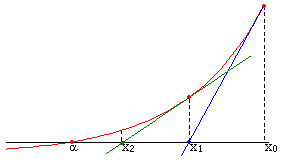
\includegraphics[width=0.55\linewidth]{newton.png}
\caption{Newton's method: the tangent line at each guess $x_n$ crosses zero at the next guess $x_{n+1}$, converging toward the root. Source: Wikipedia}
\label{fig:newton-tangent}
\end{figure}

Each iteration replaces the (generally curved, transcendental) function $f$ by its local straight-line approximation and solves \emph{that} exactly --- which is why Newton's method is sometimes described as ``linearize and solve, repeatedly.''

For our residual, Eq.~\eqref{eq:residual}, the derivative needed at every iteration is
\begin{equation}
f'(V) = \frac{\dd \tau_{\mathrm{friction}}}{\dd V} = \frac{\sigma_n a}{V},
\label{eq:fprime}
\end{equation}
where the derivative is taken holding $\theta$ fixed, consistent with the remark in Section~3.1: throughout the entire Newton iteration, $\theta$ sits still at its current value, and only $V$ moves from one iterate to the next. Because $f'$ is available in closed form here, each Newton iteration costs one evaluation of $f$ and one of $f'$ --- both $\order{1}$ operations.

\subsection{Algorithm}

\begin{center}
\fbox{\begin{minipage}{0.9\linewidth}
\textbf{Newton--Raphson for $f(V)=0$}
\begin{enumerate}[label=\arabic*.]
\item Choose an initial guess $V_0$ and a tolerance $\varepsilon$.
\item For $n = 0, 1, 2, \dots$:
\begin{enumerate}[label=(\alph*)]
\item Evaluate $f(V_n)$ and $f'(V_n)$.
\item Update: $V_{n+1} = V_n - f(V_n)/f'(V_n)$.
\item If $|V_{n+1} - V_n| < \varepsilon$ (or $|f(V_{n+1})| < \varepsilon$), stop and accept $V_{n+1}$.
\end{enumerate}
\item If a maximum iteration count is reached without convergence, flag failure (see Section~4.6).
\end{enumerate}
\end{minipage}}
\end{center}

\subsection{Convergence theory}

The appeal of Newton's method is not just that it works, but that --- under the right conditions --- it works \emph{very} fast.

Here is the intuition, without the formalism. Look again at Figure~\ref{fig:newton-tangent}: each tangent-line step landed noticeably closer to the root than the step before. That is not a coincidence of this particular curve --- it is a general feature of using a \emph{curved} function's tangent line as an approximation. The further you are from the root, the more the curve bends away from its tangent line, so a tangent-line step from far away is a poor approximation and can land almost anywhere. But once you are \emph{close} to the root, the curve is almost indistinguishable from its own tangent line over that short remaining distance, so the tangent-line step is almost exactly right. The error left over is only due to how much the curve bends (its curvature, $f''$) over that short remaining distance --- and that leftover error is proportional to the \emph{square} of how far off you already were. Being twice as close to the root, roughly speaking, makes the next step four times closer still.

This is the entire content of what a textbook would call Newton's ``quadratic convergence'' guarantee: \emph{once you are close enough to a root}, the number of correct decimal digits roughly \emph{doubles} every iteration. If $V_n$ is off by about $10^{-1}$, expect $V_{n+1}$ off by about $10^{-2}$, $V_{n+2}$ off by about $10^{-4}$, and $V_{n+3}$ off by about $10^{-8}$ --- machine precision, in three or four more steps. This is why, in practice, well-posed Newton iterations for smooth friction laws converge to machine precision in 3--5 iterations.

The catch is the phrase \emph{once you are close enough}: nothing above promises fast (or any) convergence starting from far away, especially wherever the curve is close to flat --- there, the tangent line barely tilts, and the ``obvious'' step can rocket past the root instead of homing in on it. We come back to exactly this failure mode, with real numbers, in Problems~1--3 of the practice problems at the end of these notes.

\subsection{A worked example}

Take, for illustration, $\sigma_n = 100\ \mathrm{MPa}$, $a = 0.010$, $b = 0.015$, $V^\ast = 10^{-6}\ \mathrm{m/s}$, $\mu^\ast = 0.6$, $\Dc = 10\ \mu\mathrm{m}$, and suppose at some instant $\theta = \Dc/V^\ast$ (i.e.\ steady state at $V^\ast$) and $\tau_{\mathrm{applied}} = 61\ \mathrm{MPa}$. The residual is
\begin{equation}
f(V) = 100\left[0.6 + 0.010\ln\!\left(\frac{V}{10^{-6}}\right) + 0.015 \ln(1)\right] - 61 = 100\left[0.6 + 0.010\ln\!\left(\frac{V}{10^{-6}}\right)\right] - 61,
\end{equation}
in MPa, with $V$ in m/s. Starting from $V_0 = 10^{-6}\ \mathrm{m/s}$: $f(V_0) = 100(0.6) - 61 = -1$ MPa, $f'(V_0) = \sigma_n a / V_0 = 100 \times 0.010 / 10^{-6} = 10^6$ MPa$\cdot$s/m. One Newton step gives
\begin{equation}
V_1 = 10^{-6} - \frac{-1}{10^6} = 10^{-6} + 10^{-6} = 2\times 10^{-6}\ \mathrm{m/s}.
\end{equation}
Evaluating $f(V_1) = 100[0.6 + 0.010\ln 2] - 61 \approx 100(0.6069) - 61 \approx -0.31$ MPa: the residual has shrunk by roughly a factor of three, consistent with rapid convergence once close to a root of a well-scaled problem. A second iteration would reduce the residual by a comparable factor again, and the iteration converges to $V^\ast \approx 2.72\times 10^{-6}\ \mathrm{m/s}$ (i.e.\ $\ln(V^\ast/10^{-6}) = 1$) within a handful of steps.

\subsection{Practical reparametrization: solving in $\ln V$}

The worked example above was gentle: the initial guess was already within one order of magnitude of the root. In an earthquake-cycle simulation, this is \emph{not} generally true --- recall from Section~2.4 that $V$ can range over nine or ten orders of magnitude over a single cycle, and the value of $V$ from the previous time step (the natural initial guess for the current step) is a poor predictor of the new $V$ precisely during the most interesting part of the cycle, the nucleation and coseismic phases, when $V$ is changing fastest.

Solving directly for $V$ has two related problems:
\begin{enumerate}
\item \textbf{Unphysical overshoot.} Nothing in the Newton update, Eq.~\eqref{eq:newton}, prevents $V_{n+1}$ from being negative. Since $f'(V) = \sigma_n a/V \to \infty$ as $V \to 0^+$, a poorly scaled step near small $V$ can easily overshoot past zero into $V<0$, where the friction law itself is undefined (the logarithm has no real argument).
\item \textbf{Badly scaled steps across decades.} $f'(V) \propto 1/V$, so the ``natural'' Newton step size $f(V_n)/f'(V_n)$ scales like $V_n$ itself. A step appropriate near $V \sim 1\ \mathrm{m/s}$ is absurdly large near $V \sim 10^{-9}\ \mathrm{m/s}$, and vice versa.
\end{enumerate}

The standard fix is to solve for the \emph{logarithm} of velocity rather than velocity itself. Define
\begin{equation}
x \equiv \ln\!\left(\frac{V}{V^\ast}\right), \qquad V = V^\ast e^{x}.
\end{equation}
Substituting into Eq.~\eqref{eq:residual} gives a new residual, linear in $x$ inside the friction term:
\begin{equation}
g(x) \equiv \sigma_n\left[\mu^\ast + a\,x + b \ln\!\left(\frac{\theta V^\ast}{\Dc}\right)\right] - \tau_{\mathrm{applied}} = 0,
\end{equation}
with derivative $g'(x) = \sigma_n a$, a \emph{constant}. Two benefits follow immediately.
\begin{itemize}
\item $V = V^\ast e^x$ is positive for \emph{any} real $x$: reparametrizing in $\log$-space makes unphysical negative velocities structurally impossible, regardless of how large a step Newton takes.
\item Because $g'$ no longer depends on $V$, Newton steps in $x$-space are naturally well-scaled across the entire dynamic range of $V$: a step of a given size in $x$ corresponds to a \emph{multiplicative} change in $V$, which is exactly the kind of change we expect as $V$ ranges over decades.
\end{itemize}
In this particular residual $g$ is in fact exactly linear in $x$ once $\theta$ is held fixed, so a single Newton step in $x$ would converge exactly; the value of the reparametrization becomes more pronounced once this root-find is embedded inside the fully coupled system of Section~8 and, later, the thermal-pressurization-coupled system of Session 5, where $\theta$ (or the effective normal stress) also depends on $V$ and the combined residual is no longer exactly linear in any single variable.

\subsection{Failure modes and remedies}

Even with the log-$V$ reparametrization, Newton's method can fail to converge, and it is worth knowing the standard symptoms and remedies, because a simulation that silently returns a garbage $V$ is far worse than one that visibly crashes.

\begin{remark}[A derivative-free alternative]
Newton's method requires $f'$ at every iteration; Eq.~\eqref{eq:fprime} gave us this in closed form, but for more complicated residuals later in the course (once thermal pressurization and dilatancy are coupled in) an analytic derivative may be inconvenient or unavailable. The \textbf{secant method} replaces $f'(V_n)$ with a finite-difference approximation built from the two most recent iterates,
\begin{equation}
V_{n+1} = V_n - f(V_n)\,\frac{V_n - V_{n-1}}{f(V_n)-f(V_{n-1})},
\end{equation}
trading Newton's quadratic convergence rate for the slightly slower superlinear rate $|e_{n+1}| \sim C|e_n|^{\varphi}$ with $\varphi = (1+\sqrt5)/2 \approx 1.618$ (the golden ratio), in exchange for needing only one new function evaluation per step rather than one function \emph{and} one derivative evaluation. We will use Newton's method throughout this course, since our residuals will always have accessible analytic derivatives, but it is worth knowing the secant method exists for the day you encounter a residual that does not.
\end{remark}

\begin{itemize}
\item \textbf{Poor initial guess.} If $x_0$ is far from the root, the local convergence theorem of Section~4.3 gives no guarantee; the iteration can wander before (if ever) entering the basin of quadratic convergence. \emph{Remedy:} use the previous time step's converged $V$ as the initial guess (warm starting), and fall back to a bisection or bracketing step if Newton diverges.
\item \textbf{Oscillation or divergence.} Near an inflection point or where $f'$ is small, Newton steps can overshoot repeatedly without converging. \emph{Remedy:} step damping (take a fraction of the Newton step, e.g.\ $V_{n+1} = V_n + \alpha \Delta V$ with $\alpha < 1$, increasing $\alpha$ toward 1 as the residual shrinks) or a line-search that only accepts a step if it reduces $|f|$.
\item \textbf{Stagnation at machine precision.} Once $|f(V_n)|$ is comparable to floating-point round-off in the evaluation of $f$, further iterations do not reduce the error and may even increase it. \emph{Remedy:} stop when the residual stops decreasing meaningfully, not only when it is exactly below a fixed tolerance.
\end{itemize}

%======================================================================
\section{Ordinary Differential Equations and Explicit Euler}
%======================================================================

\subsection{The initial value problem}

Newton's method solves an algebraic equation at a single instant. But $\tau$ and $\theta$ in our spring-slider system evolve continuously in time, governed by the coupled ODEs, Eqs.~\eqref{eq:loading} and~\eqref{eq:aging}. In general we consider an initial value problem (IVP)
\begin{equation}
\frac{\dd y}{\dd t} = f(t, y), \qquad y(t_0) = y_0,
\label{eq:ivp}
\end{equation}
where $y$ may be a scalar or, as in our case, a vector of state variables ($\tau$ and $\theta$ together). We seek a numerical approximation $y_n \approx y(t_n)$ at a sequence of discrete times $t_0 < t_1 < t_2 < \dots$, typically with a fixed step $h = t_{n+1}-t_n$ (though adaptive step sizing, previewed in Section~6.9, will vary $h$).

\subsection{Euler's method, from a Taylor expansion}

The simplest numerical integrator follows from truncating a Taylor expansion of $y$ about $t_n$:
\begin{equation}
y(t_n + h) = y(t_n) + h\,y'(t_n) + \tfrac{1}{2}h^2 y''(t_n) + \order{h^3} = y(t_n) + h\,f(t_n, y(t_n)) + \order{h^2}.
\end{equation}
Dropping the $\order{h^2}$ remainder and replacing the (unknown) exact solution $y(t_n)$ by its numerical approximation $y_n$ defines the \textbf{explicit (forward) Euler method}:
\begin{equation}
\boxed{\, y_{n+1} = y_n + h\, f(t_n, y_n) \,}.
\label{eq:euler}
\end{equation}
It is the numerical-integration analogue of Newton's method: a local, first-order (linear) approximation of the true dynamics, applied repeatedly. In plain terms: at every step, look at which way the solution is currently heading (its slope, $f(t_n,y_n)$), and walk in a straight line in that direction for a distance $h$ --- then look again, and repeat. Figure~\ref{fig:euler-staircase} shows what this looks like against the true, curving solution: because the true solution keeps curving away from whatever straight line you're currently walking along, each step drifts a little further off track than the last.

\begin{figure}[h]
\centering
\begin{tikzpicture}[xscale=4.4, yscale=3.6]
\draw[-{Stealth[length=2mm]}] (0,0) -- (1.65,0) node[right] {\small $t$};
\draw[-{Stealth[length=2mm]}] (0,0) -- (0,1.15) node[above] {\small $y$};
% true solution y=e^{-t}
\draw[thick, blue!60!black, domain=0:1.55, samples=60, smooth] plot (\x, {exp(-\x)});
\node[blue!60!black] at (0.62,0.92) {\small true solution $y(t)=e^{-t}$};
% Euler polygon with h=0.5: y0=1, y1=0.5, y2=0.25, y3=0.125
\draw[red!70!black, thick] (0,1) -- (0.5,0.5) -- (1.0,0.25) -- (1.5,0.125);
\filldraw[black] (0,1) circle (1.1pt) node[left] {\small $y_0$};
\filldraw[black] (0.5,0.5) circle (1.1pt) node[below=1pt] {\small $y_1$};
\filldraw[black] (1.0,0.25) circle (1.1pt) node[below=1pt] {\small $y_2$};
\filldraw[black] (1.5,0.125) circle (1.1pt) node[below=1pt] {\small $y_3$};
\node[red!70!black] at (1.05,0.62) {\small Euler steps ($h=0.5$)};
\draw[dashed, gray] (1.0,0.25) -- (1.0,{exp(-1.0)});
\draw[{Stealth[length=1.5mm]}-{Stealth[length=1.5mm]}] (1.02,0.25) -- (1.02,{exp(-1.0)-0.01}) node[midway, right, black, xshift=1pt] {\footnotesize gap};
\end{tikzpicture}
\caption{Euler's method walks in a straight line along the \emph{current} slope for one full step (red segments), while the true solution (blue) keeps curving. Each step's straight-line assumption is only exactly right at its starting point, so the numerical path drifts progressively further from the truth --- here for $y'=-y$, $y(0)=1$, with a deliberately large $h=0.5$ to make the drift visible.}
\label{fig:euler-staircase}
\end{figure}

\subsection{Local and global truncation error}

Two distinct notions of error matter for any time-stepping scheme, and it is worth being clear about the difference between them, even without belaboring a formal proof.

\textbf{Local truncation error} is the error made by a \emph{single} step, assuming that step started from the exact solution. For Euler's method, this is exactly the piece of the Taylor expansion we truncated in Section~5.2:
\begin{equation}
\tau_n \equiv y(t_{n+1}) - \left[y(t_n) + h\,f(t_n, y(t_n))\right] = \tfrac{1}{2}h^2 y''(\xi_n) = \order{h^2}.
\end{equation}
A method whose local error is $\order{h^{p+1}}$ is said to have \textbf{order} $p$; Euler's method, with local error $\order{h^2}$, has order $p=1$.

\textbf{Global error} is the accumulated discrepancy between the numerical and exact solutions after many steps, $E_n \equiv y_n - y(t_n)$, once we actually run the method for $N \sim (T-t_0)/h$ steps rather than just one. Global error is not simply $N$ times the local error added up; each step's local error also gets carried forward and reshaped by the dynamics over every subsequent step. The standard result --- true under mild conditions on $f$, and something we will confirm numerically rather than prove here (Section~8.4) --- is that this accumulation costs exactly \emph{one power of $h$}: a method with local error $\order{h^{p+1}}$ has global error $\order{h^p}$.

\begin{remark}
This one-power-of-$h$ rule of thumb is why we always describe a method by its (global) \textbf{order} $p$ rather than by the order of its local error: it is the global error, accumulated over the whole simulated time interval, that we actually care about. Euler's method, order $p=1$, has global error $\order{h}$: halving the step size only halves the error, and achieving one additional digit of accuracy requires roughly a tenfold reduction in $h$ (hence a tenfold increase in the number of, admittedly cheap, steps). This is the number to keep in mind when Section~6 introduces methods with $p=4$, where the same one-digit improvement costs far fewer extra steps.
\end{remark}

\subsection{Linear stability}

Accuracy is not the only concern; a numerical method must also be \emph{stable} for a given step size, or errors will grow rather than merely accumulate. Here is the idea in the plainest possible setting before we generalize it.

Suppose $y$ decays exponentially, $y'=\lambda y$ with $\lambda$ a negative real number, so the true solution $y(t)=y_0 e^{\lambda t}$ shrinks steadily toward zero. Apply one Euler step:
\begin{equation}
y_{n+1} = y_n + h\lambda y_n = (1+h\lambda)\,y_n.
\end{equation}
Every step just multiplies the current value by the same fixed number, $(1+h\lambda)$. That number is the whole story: if $|1+h\lambda| < 1$, repeated multiplication shrinks $y_n$ toward zero, matching the true decaying solution --- good. But if $|1+h\lambda|>1$, repeated multiplication makes $|y_n|$ \emph{grow without bound}, even though the true solution is decaying --- the numerical scheme has manufactured an instability that has nothing to do with the real physics, purely because $h$ was too large relative to $|\lambda|$. And if $1+h\lambda$ happens to be negative (which happens once $h|\lambda|>1$), the sign flips every step too, so an unstable run doesn't just grow, it \emph{oscillates} while it grows --- exactly the wild zig-zag you will compute by hand in Problem~4.

Write $z = h\lambda$ and $R(z) \equiv 1+z$ for this multiplier (the \textbf{amplification factor}). The condition for stability, $|R(z)|\le 1$, traces out a disk in the complex $z$-plane --- Euler's \textbf{region of absolute stability} --- shown in Figure~\ref{fig:euler-stability-disk}. For our purposes $\lambda$ is real and negative (a diffusive or frictionally-damped relaxation rate, not an oscillation), so all that matters is the real-axis slice of that disk: stability requires
\begin{equation}
h \le \frac{2}{|\lambda|}.
\end{equation}
The step size is bounded by the fastest-decaying mode in the system --- the more strongly damped a process is, the smaller a step Euler needs to keep up with it.

\begin{figure}[h]
\centering
\begin{tikzpicture}[scale=1.15]
\draw[-{Stealth[length=2mm]}] (-3.3,0) -- (1.3,0) node[right] {\small $\mathrm{Re}(z)$};
\draw[-{Stealth[length=2mm]}] (0,-1.7) -- (0,1.7) node[above] {\small $\mathrm{Im}(z)$};
\filldraw[blue!15] (-1,0) circle (1);
\draw[blue!60!black, thick] (-1,0) circle (1);
\filldraw[black] (-2,0) circle (1pt) node[below] {\small $-2$};
\filldraw[black] (0,0) circle (1pt) node[below right] {\small $0$};
\node[blue!60!black] at (-1,0) {\small stable};
\node at (0.55,1.35) {\small unstable out here};
\end{tikzpicture}
\caption{Euler's region of absolute stability: the shaded disk $|1+z|\le1$, $z=h\lambda$. For real, negative $\lambda$, this is exactly the segment $-2\le z \le 0$, i.e.\ $h\le 2/|\lambda|$.}
\label{fig:euler-stability-disk}
\end{figure}

\begin{remark}
This is exactly the concern flagged in Session 5: once frictional heating and thermal pressurization couple into the spring-slider system, the effective $|\lambda|$ of the fastest mode grows sharply once slip accelerates, forcing Euler's step size down catastrophically at precisely the moment the simulation is most expensive to run. This is why the coupled system will eventually need either an implicit method or, at minimum, a higher-order explicit method with adaptive step control --- the subject of the rest of this section and Section~6.9.
\end{remark}

\subsection*{A short digression: why stiffness, and why eigenvalues?}

Problems 4--6 all turn on the same underlying idea, so it's worth pausing to build it properly before diving in --- not just naming it, but seeing where it actually comes from.

\paragraph{The question a coupled system raises.} Section~5.4 analyzed exactly one scalar equation, $y'=\lambda y$, and got a clean stability bound: $h\le 2/|\lambda|$. But our real system isn't scalar --- $\tau$ and $\theta$ push on each other, and soon (Session~5) temperature and pore pressure will too. The natural question is: where does a single number like $\lambda$ come from once the equations are coupled? Is there even such a number?

\paragraph{Locally, a coupled system isn't really coupled.} The resolution is the same move used everywhere else in these notes: linearize. Near any given state $\mathbf y_0$, a nonlinear system $\mathbf y' = \mathbf f(\mathbf y)$ looks, for small deviations $\delta\mathbf y = \mathbf y - \mathbf y_0$, like the linear system
\begin{equation}
\delta\mathbf y' \;\approx\; J\,\delta\mathbf y, \qquad J \equiv \left.\frac{\partial \mathbf f}{\partial \mathbf y}\right|_{\mathbf y_0},
\end{equation}
the Jacobian of $\mathbf f$ evaluated at the current state --- exactly the multivariable version of the single derivative $f'(V_n)$ that drove Newton's method in Section~4. And a linear system, however coupled it looks written out in the original variables, is secretly just several \emph{independent} scalar equations wearing a disguise: change coordinates to the eigenvectors of $J$, and each component $z_i$ of $\delta\mathbf y$ in that basis evolves completely on its own,
\begin{equation}
z_i' = \lambda_i z_i,
\end{equation}
one copy of Section~5.4's scalar test equation per eigenvalue $\lambda_i$ of $J$. Nothing here is a linear-algebra abstraction bolted onto the problem --- the eigenvalues are the decay (or growth) rates of the system's own natural, hidden, independent directions. A system with $m$ state variables generically has $m$ such directions, each ticking at its own rate, and you only see them once you look along the right axes.

\paragraph{Why this controls the step size.} A numerical method has no idea this hidden decomposition exists --- it just applies the same update rule to the whole vector $\mathbf y$ every step. But because the decomposition is linear, the method's action on $\delta\mathbf y$ splits the same way: it is, invisibly, applying the scalar Euler (or RK4) update to \emph{every} mode $z_i$ at once, superimposed. Stability of the whole system requires stability on \emph{every} mode simultaneously, and a chain is only as strong as its weakest link: the step-size bound is set by whichever $\lambda_i$ has the largest $|\mathrm{Re}(\lambda_i)|$ ---
\begin{equation}
h \;\lesssim\; \frac{2}{\max_i |\mathrm{Re}(\lambda_i)|},
\end{equation}
even if that particular mode is a minor, fast-decaying, physically-uninteresting-by-now piece of the solution. The slow modes you actually care about resolving are just along for the ride, throttled by a clock that has nothing to do with them.

\paragraph{A semi-formal definition.} This gives a working criterion for \textbf{stiffness}. Define the \textbf{stiffness ratio}
\begin{equation}
S \;=\; \frac{\max_i |\mathrm{Re}(\lambda_i)|}{\min_i |\mathrm{Re}(\lambda_i)|}
\end{equation}
of the Jacobian $J$ (restricting to eigenvalues with $\mathrm{Re}(\lambda_i)<0$, the decaying modes relevant to diffusive and frictional relaxation). A system is called stiff, for a given explicit method, when \emph{both}:
\begin{enumerate}[label=(\roman*)]
\item $S \gg 1$ --- the decay rates are widely separated, \emph{and}
\item the interval you need to integrate over is comparable to the \emph{slow} mode's own timescale, $1/\min_i|\mathrm{Re}(\lambda_i)|$ --- i.e.\ the fast mode isn't what you actually need resolved; it may have already settled down.
\end{enumerate}
When both hold, stability --- not accuracy --- is what's throttling your step size, for a mode you've already stopped caring about. That is the actual bite of stiffness: it is not a statement about how hard a problem is to get right, but about which constraint (stability or accuracy) is binding.

\begin{remark}
This eigenvalue-ratio criterion is a \emph{working} definition, useful and standard, but not a universally agreed rigorous one --- stiffness has famously resisted a single clean formalization since the term was coined. Curtiss and Hirschfelder's original 1952 paper defines it almost operationally: a problem is stiff if explicit methods need impractically small steps to stay stable, while implicit methods (Section~6.11) do not. The eigenvalue ratio $S$ is the standard way to make that operational statement checkable in advance, not a competing definition.
\end{remark}

\paragraph{Where we stand today.} Right now, with only $\tau$ and $\theta$ as state variables, there is really just one relaxation clock in play --- $\theta$'s own rate $|\lambda|\approx V/D_c$, the quantity you compute in Problem~6 --- so $S$ isn't yet meaningfully defined; a \emph{ratio} needs at least two rates to compare. The moment Session~5 adds a diffusive temperature/pressure state with its own decay rate, the Jacobian becomes genuinely multi-eigenvalue, and that is the first point at which ``eigenvalues,'' plural, stops being overkill notation and becomes the actual object governing the step size.

\begin{center}
\fbox{\begin{minipage}{0.92\linewidth}
\textbf{A quick practical diagnostic}
\begin{itemize}
\item Estimate $h_{\mathrm{acc}}$: the step size accuracy alone would ask for, to resolve the solution's actual features.
\item Estimate $h_{\mathrm{stab}} \sim 2/\max_i|\mathrm{Re}(\lambda_i)|$: the step size your method's stability region permits, using the \emph{fastest} decaying mode anywhere in the system.
\item If $h_{\mathrm{stab}} \ll h_{\mathrm{acc}}$, the problem is stiff for that method: you're forced into far more steps than the solution's own behavior would ever require, purely to keep the fast mode from blowing up numerically.
\end{itemize}
\end{minipage}}
\end{center}

Problem~6 is the version of this that matters for the rest of the course: the friction state variable relaxes at a rate $|\lambda|\approx V/D_c$ that is itself part of the solution, and swings across nine orders of magnitude between the interseismic and coseismic phases of a single earthquake cycle. The system is mild (or not stiff at all) while creeping, and becomes extremely stiff the moment slip accelerates --- which is exactly why a single fixed step size can never be both safe and efficient across a full cycle, and why the coupled model of Session~5 will need either adaptive step control (Section~6.10) or an implicit method (Section~6.11), rather than the fixed-step RK4 that suffices for today's dry spring-slider.

%======================================================================
\section{Runge--Kutta Methods}
%======================================================================

\subsection{Motivation}

Euler's method uses the derivative $f(t_n, y_n)$ evaluated at a single point --- the start of the step --- and extrapolates linearly across the whole interval $[t_n, t_{n+1}]$. If $f$ varies substantially across that interval (which it will, whenever the dynamics are fast relative to $h$), a single-point estimate of the slope is a poor representative of the average slope needed to get from $y_n$ to $y_{n+1}$ accurately. This is exactly the drift you saw in Figure~\ref{fig:euler-staircase}: the slope Euler commits to at the start of the step is already stale by the end of it.

The idea behind Runge--Kutta (RK) methods is simply: sample the slope at \emph{several} points across the step instead of just one, and combine the samples into a better estimate of the average slope. Figure~\ref{fig:rk4-stages} previews what this looks like for the specific 4-point scheme we derive in Section~6.6: sample once at the start of the step, twice near the middle (each time with a better guess of where the solution actually is by then), and once at the end, then take a weighted average of all four. Critically, this is achieved \emph{without} needing derivatives of $f$ itself (unlike, say, a Taylor-series method that would require $f$, $f_t + f_y f$, and so on); only evaluations of $f$ at various $(t,y)$ pairs are needed, which is exactly what makes RK methods practical for the nonlinear, closed-form-derivative-free right-hand sides we will build later in the semester.

\begin{figure}[h]
\centering
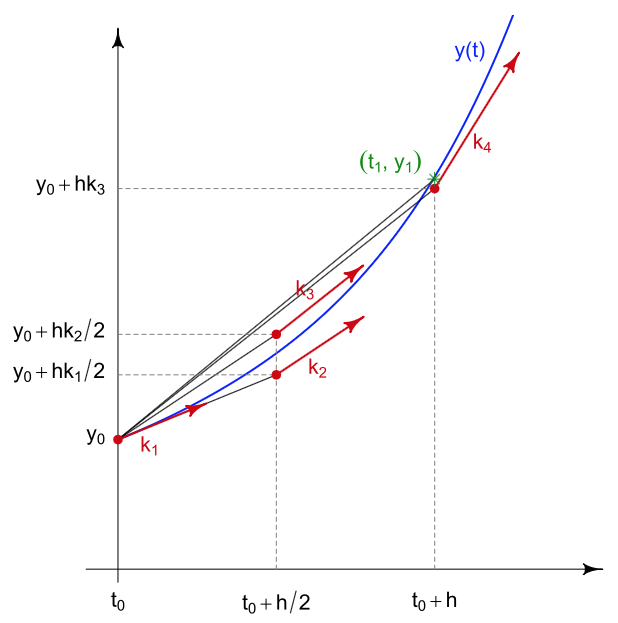
\includegraphics[width=0.5\linewidth]{rk.png}
\caption{Where RK4 samples the slope within one step: once at the start, twice near the midpoint (using progressively better predictions of where the solution is by then), and once at the end. The final update (Section~6.6) averages these four, weighting the two midpoint samples twice as heavily as the two endpoint samples. Source: Wikipedia}
\label{fig:rk4-stages}
\end{figure}

\subsection{The general explicit $s$-stage formula}

An explicit Runge--Kutta method with $s$ \textbf{stages} computes $s$ intermediate slope estimates $k_1, \dots, k_s$, each depending only on \emph{previously computed} stages (hence ``explicit''), and combines them into the update:
\begin{align}
k_i &= f\!\left(t_n + c_i h,\; y_n + h\sum_{j=1}^{i-1} a_{ij}\,k_j\right), \qquad i = 1, \dots, s, \label{eq:rk-stages}\\
y_{n+1} &= y_n + h\sum_{i=1}^{s} b_i\,k_i. \label{eq:rk-update}
\end{align}
The coefficients $a_{ij}$ (for $j < i$), $b_i$, and $c_i$ fully specify the method. Different choices of these coefficients, subject to certain consistency and order conditions (Section~6.4), give different named methods --- Euler's method is the degenerate $s=1$ case ($a$ empty, $b_1=1$, $c_1=0$); the classical fourth-order method of Section~6.6 is the $s=4$ case most students associate with the name ``Runge--Kutta.''

\subsection{The Butcher tableau}

The coefficients of an RK method are conventionally organized into a compact array called the \textbf{Butcher tableau} (Butcher, 1964), named for the numerical analyst John C.\ Butcher:
\begin{equation}
\begin{array}{c|c}
\mathbf{c} & A \\ \hline
 & \mathbf{b}^{\mathsf T}
\end{array}
\quad = \quad
\begin{array}{c|cccc}
c_1 & & & & \\
c_2 & a_{21} & & & \\
\vdots & \vdots & \ddots & & \\
c_s & a_{s1} & \cdots & a_{s,s-1} & \\ \hline
 & b_1 & \cdots & b_{s-1} & b_s
\end{array}
\end{equation}
where $A = (a_{ij})$ is a \emph{strictly lower triangular} $s\times s$ matrix for an explicit method (the entries $a_{ij}$ for $j \ge i$ are simply absent, or equivalently zero, which is precisely what makes the stage computation~\eqref{eq:rk-stages} explicit rather than requiring a nonlinear solve at each stage), $\mathbf{b} = (b_1,\dots,b_s)^{\mathsf T}$ are the stage weights that appear in the final update~\eqref{eq:rk-update}, and $\mathbf{c} = (c_1,\dots,c_s)^{\mathsf T}$ are the fractional locations, within the step, at which each stage's slope is evaluated.

The tableau is not merely a bookkeeping convenience: every property of the method we will discuss below --- consistency, order, and linear stability --- can be read directly off $(A, \mathbf b, \mathbf c)$, which is why the tableau, rather than the explicit stage formulas, is the standard way numerical analysts communicate and compare RK methods.

\subsection{Consistency and order conditions}

For the method to make sense at all, the stage evaluated at fractional time $c_i$ needs to be evaluated using a $y$-estimate appropriate to that fractional time --- you can't sample the slope at the midpoint of the step using a $y$-value that only advanced a quarter of the way there. This bookkeeping requirement, the \textbf{row-sum condition},
\begin{equation}
c_i = \sum_{j=1}^{i-1} a_{ij}, \qquad i = 1,\dots, s,
\label{eq:rowsum}
\end{equation}
is automatically satisfied by every tableau below, and it's standard practice to simply read $c_i$ off the row sums of $A$ rather than specify it independently.

Beyond that bookkeeping, getting a method to actually be accurate to a given order takes more: the coefficients must satisfy a handful of algebraic conditions, the \textbf{order conditions}, obtained by writing out the true solution and the numerical update as power series in $h$ and demanding they agree term by term, as far as you want the order to reach. The first three are:
\begin{align}
\text{order } 1 \text{ (consistency):} &\quad \sum_{i=1}^s b_i = 1, \label{eq:order1}\\
\text{order } 2: &\quad \sum_{i=1}^s b_i c_i = \frac{1}{2}, \label{eq:order2}\\
\text{order } 3: &\quad \sum_{i=1}^s b_i c_i^2 = \frac{1}{3}, \qquad \sum_{i,j} b_i a_{ij} c_j = \frac{1}{6}. \label{eq:order3}
\end{align}
Order 1 (Eq.~\eqref{eq:order1}) just says the weights $b_i$ average to a full step: applied to the trivial ODE $y'=1$, the method must reproduce the exact answer $y_{n+1}=y_n+h$ --- the bare minimum for calling something a numerical integrator at all. Euler's method ($s=1$, $b_1=1$) satisfies this but not Eq.~\eqref{eq:order2} (since $c_1=0$ gives $b_1c_1=0\ne\tfrac12$), consistent with it being only first order.

\paragraph{Where the order-2 condition comes from (optional derivation).} It's worth seeing this worked out once, so the conditions above stop looking like they fell from the sky. For a general 2-stage method, write out $k_2$'s Taylor expansion for small $h$, substitute into the update $y_{n+1}$, and compare against the true solution's own Taylor expansion (using $y'=f$ and $y''=f_t+ff_y$ from the chain rule). Matching the $h^1$ terms of the two expansions gives $b_1+b_2=1$; matching the $h^2$ terms gives $b_2c_2=\tfrac12$ --- exactly Eqs.~\eqref{eq:order1}--\eqref{eq:order2}. This is the general recipe behind every order condition at every order: expand both sides in powers of $h$, and force them to agree.

The number of these conditions grows fast --- 1 at order 1, 1 more at order 2, 2 more at order 3, 4 more at order 4 (8 total), 17 by order 5 --- simply because there are more and more distinct ways for the chain rule to combine $f$ and its derivatives the further out you expand. Fully organizing and generating them at high order is the subject of a nice piece of mathematics (Butcher's ``rooted tree'' theory) that we won't need here; we will simply use tableaus, like the ones below, that are already known to satisfy all the conditions up to the stated order. The one fact worth remembering is that it is possible to satisfy all 8 order-4 conditions with only 4 stages --- no wasted effort --- which is exactly what makes the classical RK4 method of Section~6.6 so effective for its cost.

\subsection{Second-order methods}

We build intuition with two of the simplest RK methods beyond Euler, both using $s=2$ stages and both satisfying the order-1 and order-2 conditions, Eqs.~\eqref{eq:order1}--\eqref{eq:order2}, but not order 3.

\paragraph{Explicit midpoint method.} Evaluate the slope once at $t_n$ to estimate $y$ at the \emph{midpoint} of the interval, then use the slope \emph{at that midpoint} for the full step:
\begin{equation}
k_1 = f(t_n, y_n), \qquad k_2 = f\!\left(t_n+\tfrac{h}{2},\, y_n + \tfrac{h}{2}k_1\right), \qquad y_{n+1} = y_n + h\,k_2.
\end{equation}
Its Butcher tableau is
\begin{equation}
\begin{array}{c|cc}
0 & & \\
1/2 & 1/2 & \\ \hline
 & 0 & 1
\end{array}
\end{equation}
Check: $\sum b_i = 0+1=1$ (order 1, Eq.~\eqref{eq:order1}); $\sum b_i c_i = 0\cdot 0 + 1\cdot\tfrac12 = \tfrac12$ (order 2, Eq.~\eqref{eq:order2}). Both are satisfied, confirming this is a second-order method built from only two function evaluations.

\paragraph{Heun's method (explicit trapezoidal / improved Euler).} Evaluate the slope at both endpoints of the interval --- using a preliminary (first-order accurate) Euler prediction for the endpoint value of $y$ --- and average the two slopes:
\begin{equation}
k_1 = f(t_n, y_n), \qquad k_2 = f(t_n + h,\, y_n + h k_1), \qquad y_{n+1} = y_n + \tfrac{h}{2}(k_1 + k_2).
\end{equation}
Its Butcher tableau is
\begin{equation}
\begin{array}{c|cc}
0 & & \\
1 & 1 & \\ \hline
 & 1/2 & 1/2
\end{array}
\end{equation}
Check: $\sum b_i = \tfrac12+\tfrac12=1$; $\sum b_i c_i = \tfrac12\cdot 0 + \tfrac12\cdot 1 = \tfrac12$. Again both order conditions are satisfied. Both the midpoint method and Heun's method are second order and cost 2 function evaluations per step, but they are \emph{different} methods (different tableaus), with different stability properties and different behavior on any given nonlinear problem --- a first illustration of the fact, developed further below, that a given order does not determine a method uniquely.

\paragraph{The one-parameter family of second-order, 2-stage methods.} In fact, the midpoint method and Heun's method are just two members of an entire family. For a general 2-stage explicit method with $c_2 = a_{21}$ free, the order-1 and order-2 conditions, $b_1+b_2=1$ and $b_2 c_2 = \tfrac12$, are \emph{two} equations in \emph{three} unknowns ($b_1,b_2,c_2$), so they determine a one-parameter family of solutions,
\begin{equation}
b_2 = \frac{1}{2c_2}, \qquad b_1 = 1 - \frac{1}{2c_2}, \qquad c_2 \neq 0 \text{ free},
\end{equation}
parametrized by the choice of $c_2 \in (0,1]$ (values outside this range are possible but rarely useful). Setting $c_2 = \tfrac12$ recovers the midpoint method ($b_1=0, b_2=1$); setting $c_2=1$ recovers Heun's method ($b_1=b_2=\tfrac12$); setting $c_2 = \tfrac23$ gives \emph{Ralston's method} ($b_1=\tfrac14, b_2=\tfrac34$), which minimizes a bound on the leading third-order error term among this family and is, in that specific sense, the ``best'' second-order 2-stage method. This is the general pattern seen again at order 4 (Sections~6.6--6.7): the order conditions constrain but do not uniquely determine a method, and different members of a given order/stage family trade off differently on stability, error-constant size, and other secondary properties.

\subsection{The classical fourth-order method (RK4)}

The method usually meant when people say simply ``Runge--Kutta,'' and the one you will implement in the coding session, uses $s=4$ stages:
\begin{align}
k_1 &= f(t_n,\, y_n),\\
k_2 &= f\!\left(t_n+\tfrac{h}{2},\, y_n+\tfrac{h}{2}k_1\right),\\
k_3 &= f\!\left(t_n+\tfrac{h}{2},\, y_n+\tfrac{h}{2}k_2\right),\\
k_4 &= f\!\left(t_n+h,\, y_n+h\,k_3\right),\\
y_{n+1} &= y_n + \frac{h}{6}\left(k_1 + 2k_2 + 2k_3 + k_4\right).
\end{align}
Read as a narrative rather than a formula: $k_1$ is the slope at the start of the step; $k_2$ uses that slope to step halfway, and re-evaluates the slope there; $k_3$ re-evaluates the slope at the midpoint \emph{again}, but now using the (presumably better) estimate of $y$ at the midpoint supplied by $k_2$; and $k_4$ uses $k_3$ to step all the way to the end of the interval and evaluates the slope there. The final update is a weighted average of these four slope estimates, with the two midpoint estimates ($k_2, k_3$) weighted twice as heavily as the two endpoint estimates ($k_1, k_4$) --- reminiscent of Simpson's rule for numerical quadrature, which weights function values at the midpoint of an interval four times as heavily as the endpoints, for exactly analogous reasons (both are constructed to be exact for cubic polynomials).

Its Butcher tableau is
\begin{equation}
\begin{array}{c|cccc}
0 & & & & \\
1/2 & 1/2 & & & \\
1/2 & 0 & 1/2 & & \\
1 & 0 & 0 & 1 & \\ \hline
 & 1/6 & 1/3 & 1/3 & 1/6
\end{array}
\end{equation}
As a partial check of the order-4 claim, verify the order-1 and order-2 conditions directly: $\sum b_i = \tfrac16+\tfrac13+\tfrac13+\tfrac16 = 1$; and with $c = (0,\tfrac12,\tfrac12,1)$, $\sum b_i c_i = \tfrac16(0) + \tfrac13(\tfrac12)+\tfrac13(\tfrac12)+\tfrac16(1) = \tfrac16+\tfrac16+\tfrac16 = \tfrac12$. Both hold, as required; verifying the remaining six order-4 conditions is a mechanical (if tedious) exercise in the same spirit, and is the content of the classical derivation due to Kutta (1901).

RK4 costs 4 function evaluations per step (versus 1 for Euler) but achieves local truncation error $\order{h^5}$ and global error $\order{h^4}$ (versus $\order{h^2}$ and $\order{h}$ for Euler, Section~5.3) --- for smooth problems, a dramatically better accuracy-per-step-size trade, which is why it is the default workhorse explicit integrator in scientific computing, and why it is the integrator you will build and use for the spring-slider model in Section~8.

\subsection{A fully worked RK4 step}

To make the abstract stage formulas concrete, work through one complete step by hand on a test problem with a known exact solution: $y' = -2ty$, $y(0)=1$, whose exact solution is $y(t)=e^{-t^2}$. Take $h=0.2$ and step from $t_0=0$, $y_0=1$ to $t_1=0.2$.

\begin{align}
k_1 &= f(t_0, y_0) = -2(0)(1) = 0,\\
k_2 &= f\!\left(t_0+\tfrac{h}{2},\, y_0+\tfrac{h}{2}k_1\right) = f(0.1,\, 1 + 0.1\times 0) = -2(0.1)(1) = -0.2,\\
k_3 &= f\!\left(t_0+\tfrac{h}{2},\, y_0+\tfrac{h}{2}k_2\right) = f(0.1,\,0.98) = -2(0.1)(0.98) = -0.196,\\
k_4 &= f\!\left(t_0+h,\, y_0+h\,k_3\right) = f(0.2,\,0.9608) = -2(0.2)(0.9608) = -0.38432,\\
y_1 &= y_0 + \frac{h}{6}\left(k_1+2k_2+2k_3+k_4\right) = 1 + \frac{0.2}{6}\big(0 - 0.4 - 0.392 - 0.38432\big) \approx 1 - 0.03881 = 0.96119.
\end{align}
Compare against the exact value $y(0.2) = e^{-0.04} \approx 0.96079$: the RK4 estimate is accurate to about $4\times 10^{-4}$ after a single step of size $h=0.2$ --- for comparison, one Euler step from the same starting point gives $y_1^{\mathrm{Euler}} = y_0 + h\,k_1 = 1 + 0.2\times 0 = 1$, an error of about $4\times 10^{-2}$, roughly \emph{one hundred times} worse, from a single function evaluation instead of four. This hundredfold gap for a hundredfold-cheaper method is, admittedly, an unusually dramatic illustration (it occurs here because $k_1=0$ exactly, so Euler's first step captures none of the local curvature at all), but it is directionally exactly what Sections~5.3 and~6.6 predict, and it is the calculation you should reproduce as a first sanity check on your own RK4 implementation in the coding session: pick any test problem with a known solution, do one step by hand, and compare against your code's output before trusting it on the friction-coupled system.

\subsection{Kutta's 3/8 rule: a second 4th-order method}

It is worth seeing at least one other 4-stage, order-4 method, if only to underline that RK4 is not the unique way to achieve fourth-order accuracy with four stages --- the order conditions of Section~6.4 constrain the coefficients but do not pin them down uniquely. Kutta's 3/8 rule (also due to Kutta, 1901) is
\begin{equation}
\begin{array}{c|cccc}
0 & & & & \\
1/3 & 1/3 & & & \\
2/3 & -1/3 & 1 & & \\
1 & 1 & -1 & 1 & \\ \hline
 & 1/8 & 3/8 & 3/8 & 1/8
\end{array}
\end{equation}
This method also satisfies all 8 order-4 conditions and so also achieves global error $\order{h^4}$, but with different intermediate stage locations $c=(0,\tfrac13,\tfrac23,1)$ (evenly spaced across the interval, rather than clustered at the midpoint twice) and, as a consequence, a different stability region (Section~6.8) and different behavior on stiff or oscillatory problems. In practice the classical RK4 tableau above is used far more often, largely because its stability region is slightly larger, but the existence of the 3/8 rule is a useful reminder that ``order 4'' describes a whole family of methods, not a single one.

\subsection{Linear stability of Runge--Kutta methods}

The same idea from Section~5.4 carries over directly: apply an RK method to $y'=\lambda y$, and every step again just multiplies the current value by some fixed number $R(z)$, $z=h\lambda$ --- only now $R(z)$ is a higher-degree polynomial instead of Euler's simple $1+z$, because there are more stages contributing to the update. For the classical RK4 method, working through the four stages on this test problem collapses everything down to
\begin{equation}
R_{\mathrm{RK4}}(z) = 1 + z + \frac{z^2}{2} + \frac{z^3}{6} + \frac{z^4}{24},
\end{equation}
which is simply the first five terms of the Taylor series for $e^z$ --- a nice consistency check, since matching $e^z$ to more and more terms is exactly what being higher order means (Section~6.4).

As with Euler, stability requires $|R(z)|\le1$. Figure~\ref{fig:rk4-vs-euler-stability} compares the two methods along the real axis, the case relevant to a purely decaying mode like ours: Euler's stable range ends at $z=-2$, while RK4's extends further, to about $z\approx-2.78$. In practical terms, RK4 tolerates a step size roughly $1.4\times$ larger than Euler for the same decay rate --- a welcome bonus given that RK4 was already going to be used for its accuracy, not its stability. But notice it is still a \emph{finite} range: push $h$ far enough and RK4 becomes unstable too, exactly like Euler. No explicit method escapes this; only an implicit method (Section~6.10) can be stable for \emph{every} step size.

\begin{figure}[h]
\centering
\begin{tikzpicture}[scale=1.0]
\draw[-{Stealth[length=2mm]}] (-3.4,0) -- (0.6,0) node[right] {\small $z=h\lambda$};
\draw (-2.78,0.05) -- (-2.78,-0.05);
\draw (-2,0.05) -- (-2,-0.05);
\draw (0,0.05) -- (0,-0.05);
\node[below] at (-2.78,-0.12) {\small $-2.78$};
\node[below] at (-2,-0.12) {\small $-2$};
\node[below] at (0,-0.12) {\small $0$};
\draw[very thick, red!70!black] (-2,0.35) -- (0,0.35);
\node[left, red!70!black] at (-2.05,0.35) {\small Euler};
\draw[very thick, blue!60!black] (-2.78,0.7) -- (0,0.7);
\node[left, blue!60!black] at (-2.83,0.7) {\small RK4};
\end{tikzpicture}
\caption{Where each method stays stable along the real axis (a purely decaying mode). RK4's stable range reaches further left than Euler's --- about $1.4\times$ further --- but both are bounded ranges, not the whole axis.}
\label{fig:rk4-vs-euler-stability}
\end{figure}

\subsection{Embedded pairs and adaptive step size: a preview}

Everything above uses a fixed step size $h$, chosen once and used throughout. In practice, and especially once thermal pressurization and dilatancy are coupled into the spring-slider system (Session 5), the natural time scale of the dynamics changes dramatically over an earthquake cycle: interseismic loading evolves over years, while coseismic slip can accelerate over milliseconds. A fixed $h$ small enough to resolve the coseismic phase would make the interseismic phase prohibitively (and pointlessly) expensive to simulate. What we want instead is a step size that adapts itself, growing when the solution is calm and shrinking when it isn't.

\paragraph{Getting two error estimates for the price of one.} The standard solution is an \textbf{embedded Runge--Kutta pair}: two RK methods of different order, say $p$ and $p+1$, constructed to \emph{share} the same stage evaluations $k_1,\dots,k_s$ (differing only in the weights $\mathbf b$ used to combine them), so that both a $p$-th order and a $(p{+}1)$-th order estimate of $y_{n+1}$ can be obtained from a single set of $s$ function evaluations:
\begin{equation}
y_{n+1}^{(p)} = y_n + h\sum_{i=1}^s b_i k_i, \qquad y_{n+1}^{(p+1)} = y_n + h\sum_{i=1}^s b_i^\ast k_i,
\end{equation}
using the \emph{same} $k_1,\dots,k_s$ in both sums --- only the weights $\mathbf b$ versus $\mathbf b^\ast$ differ. The difference between the two estimates,
\begin{equation}
\widehat{e}_{n+1} \;=\; y_{n+1}^{(p+1)} - y_{n+1}^{(p)} \;=\; h\sum_{i=1}^s \left(b_i^\ast - b_i\right) k_i,
\label{eq:embedded-error}
\end{equation}
is then a cheap, practical estimate of the local truncation error of the lower-order method --- cheap because it costs no extra function evaluations beyond the $s$ we were already computing.

\paragraph{Turning the error estimate into a step size.} Recall from Section~5.3 that a $p$-th order method has local error $\order{h^{p+1}}$, i.e.\ $|\widehat{e}_{n+1}| \approx C h^{p+1}$ for some constant $C$ that depends on the local behavior of the solution but not on $h$. If we specify a tolerance $\mathrm{tol}$ we want the local error to stay below, we can solve this relationship for the step size that \emph{would have} hit that tolerance exactly, and use it as our next attempt. Writing the scalar error ratio
\begin{equation}
\mathrm{err}_{n+1} \;=\; \frac{|\widehat{e}_{n+1}|}{\mathrm{tol}},
\end{equation}
(with $\mathrm{tol} = \mathrm{atol} + \mathrm{rtol}\,|y_n|$ a mix of absolute and relative tolerance, in practice), the standard step-size update is
\begin{equation}
\boxed{\, h_{\mathrm{new}} \;=\; h \cdot S \left(\frac{1}{\mathrm{err}_{n+1}}\right)^{1/(p+1)} \,}
\label{eq:step-control}
\end{equation}
where $S \approx 0.9$ is a \textbf{safety factor}, pulling back slightly from the theoretical optimum so the next step is more likely to succeed too, rather than landing right on the edge of the tolerance. In practice $h_{\mathrm{new}}$ is also clamped to a modest range around $h$ (e.g.\ never grow by more than a factor of $5$ or shrink by more than a factor of $10$ in one step), so that a single wild error estimate can't send the step size to an extreme in one jump.

\paragraph{Accept or reject.} Unlike the fixed-step algorithm of Section~8, an adaptive step is provisional until checked:
\begin{itemize}
\item If $\mathrm{err}_{n+1} \le 1$ (the error came in under tolerance), \textbf{accept} the step --- advance to $y_{n+1}^{(p+1)}$ (the higher-order estimate; this free upgrade is called \textbf{local extrapolation}) --- and use $h_{\mathrm{new}}$ from Eq.~\eqref{eq:step-control} for the \emph{next} step.
\item If $\mathrm{err}_{n+1} > 1$ (the error exceeded tolerance), \textbf{reject} the step: discard $y_{n+1}$ entirely, and retry the \emph{same} step from $y_n$ using the smaller $h_{\mathrm{new}}$ that Eq.~\eqref{eq:step-control} already computed.
\end{itemize}
Either way, no work is wasted: the same $s$ function evaluations that produced the (accepted or rejected) step also told us what step size to try next.

\begin{center}
\fbox{\begin{minipage}{0.9\linewidth}
\textbf{One adaptive step, embedded RK pair}
\begin{enumerate}[label=\arabic*.]
\item Compute stages $k_1,\dots,k_s$ once (Eq.~\eqref{eq:rk-stages}).
\item Form both estimates $y_{n+1}^{(p)}$, $y_{n+1}^{(p+1)}$ and the error estimate $\widehat{e}_{n+1}$, Eq.~\eqref{eq:embedded-error}.
\item Compute $\mathrm{err}_{n+1} = |\widehat{e}_{n+1}|/\mathrm{tol}$ and $h_{\mathrm{new}}$ from Eq.~\eqref{eq:step-control}.
\item If $\mathrm{err}_{n+1}\le 1$: accept, advance to $y_{n+1}^{(p+1)}$, move on with step size $h_{\mathrm{new}}$.
\item If $\mathrm{err}_{n+1}> 1$: reject, retry the same step from $y_n$ with step size $h_{\mathrm{new}}$.
\end{enumerate}
\end{minipage}}
\end{center}

The best-known embedded pair is the Dormand--Prince method (RK45, using a 5th- and a 4th-order estimate from 6 or 7 stages), which underlies the default adaptive ODE solvers in most scientific software (e.g.\ \texttt{scipy.integrate.solve\_ivp}'s \texttt{RK45}, MATLAB's \texttt{ode45}). We will not derive an embedded pair today, but the coupling session (Session 5) will build directly on the fixed-step RK4 method developed here, adding exactly this accept/reject/resize machinery of Eq.~\eqref{eq:step-control} once the coupled dynamics make a fixed step size impractical.

\subsection{A note on implicit methods and stiffness}

Every method presented above is \emph{explicit}: each stage $k_i$ depends only on previously computed stages, so the strictly lower-triangular structure of $A$ lets us evaluate $k_1, k_2, \dots$ one at a time, in order, with no algebraic solve beyond the friction-law root-find already embedded in each stage's right-hand side. This is what keeps the method cheap.

The alternative is an \textbf{implicit} Runge--Kutta method, in which $A$ is full (or at least not strictly lower triangular), so that $k_i$ depends on $k_j$ for $j \ge i$ as well as $j<i$ --- meaning \emph{all} the stages must, in general, be solved for \emph{simultaneously}, as a coupled system of nonlinear equations (via, unsurprisingly, a multivariate generalization of Newton's method). The simplest example is the \textbf{backward (implicit) Euler} method,
\begin{equation}
y_{n+1} = y_n + h\,f(t_{n+1}, y_{n+1}),
\end{equation}
whose Butcher tableau is the trivial $1\times1$ array $c_1=1$, $a_{11}=1$, $b_1=1$ --- note $a_{11}$ is on the diagonal, not below it, which is exactly what makes the method implicit. Applying it to the linear test equation $y'=\lambda y$ gives the amplification factor $R(z) = 1/(1-z)$, whose stability region $\{z : |1/(1-z)|\le 1\}$ is the \emph{entire left half of the complex plane}: backward Euler is stable for \emph{any} step size $h>0$ whenever $\mathrm{Re}(\lambda)\le 0$ (a property called \textbf{A-stability}), in sharp contrast to the bounded stability disks of every explicit method discussed above (Sections~5.4 and~6.8).

A closely related, and frequently used, alternative is the \textbf{trapezoidal rule} (also called Crank--Nicolson in the PDE literature), which averages the explicit and implicit Euler right-hand sides:
\begin{equation}
y_{n+1} = y_n + \frac{h}{2}\Big[f(t_n,y_n) + f(t_{n+1}, y_{n+1})\Big],
\end{equation}
with Butcher tableau
\begin{equation}
\begin{array}{c|cc}
0 & 0 & 0\\
1 & 1/2 & 1/2 \\ \hline
 & 1/2 & 1/2
\end{array},
\end{equation}
an implicit 2-stage method (note the nonzero $a_{22}=1/2$ on the diagonal of the second row) that is second order (it satisfies Eqs.~\eqref{eq:order1}--\eqref{eq:order2} by the same check as Heun's method, whose tableau it resembles but for that one diagonal entry) \emph{and} A-stable, with amplification factor $R(z) = (1+z/2)/(1-z/2)$. It is, in a sense, the implicit counterpart to Heun's method, trading Heun's conditional stability for unconditional stability at second, rather than first, order --- a strictly better stability-for-accuracy trade than backward Euler, at the cost of the same per-stage nonlinear solve.

This unconditional stability is purchased at the price of a nonlinear solve, of comparable difficulty to the friction-law root-find of Section~4, \emph{at every single stage} rather than merely embedded in evaluating an explicit right-hand side. Whether that price is worth paying is precisely a question of \textbf{stiffness}: how large is $|\lambda|$ (the fastest decay or growth rate present in the system) relative to the time scale of the dynamics you actually care about resolving? Today's dry spring-slider is not stiff, and RK4 is the right tool. Once thermal pressurization couples frictional heating to pore pressure to weakening to yet faster slip (Session~5), the fastest mode in the system accelerates sharply during the coseismic phase, and the choice between a very small explicit step and an implicit (or, more practically, a semi-implicit / adaptive-explicit) method becomes a live design decision rather than an academic one. We flag it here so that when it resurfaces in Session~5, it is a familiar idea being applied, not a new one being introduced under time pressure.

%======================================================================
\section{From Loops to Vectorized Code}
%======================================================================

\subsection{Why this matters, twice more, later}

Everything above is naturally expressed, and will be implemented in the coding session, as scalar Python functions acting on scalar (or, once we track $\tau$ and $\theta$ together, small-vector) state. That implementation effort pays for itself twice more this semester: in Sessions~3--4, assembling and repeatedly multiplying an $N\times N$ elastic stiffness matrix (one entry per pair of fault patches) is only tractable if done with vectorized array operations rather than explicit Python loops; and in Sessions~5--6, evaluating the friction law, the diffusion update, and the dilatancy relaxation together, at every one of possibly thousands of time steps, has the same requirement. Shaky vectorization habits formed now compound into real performance and readability costs later, which is why we spend a short amount of time on it today, even though it is not, strictly, numerical analysis.

\subsection{Arrays, elementwise operations, and broadcasting}

A NumPy array supports elementwise arithmetic directly: if \texttt{V} is an array of slip velocities, \texttt{k * V} multiplies every entry by the scalar \texttt{k} without an explicit loop, and \texttt{V1 - V2} subtracts two same-shaped arrays elementwise. This is not merely syntactic convenience; vectorized operations are implemented in compiled C code under the hood and are typically one to two orders of magnitude faster than the equivalent explicit \texttt{for} loop in pure Python, for array sizes of practical interest.

\textbf{Broadcasting} is the rule that lets NumPy combine arrays of different (but compatible) shapes without the user manually replicating data: a scalar combines with an array of any shape; more generally, two array shapes are compatible if, comparing dimensions from the right, each pair of dimensions is either equal or one of them is 1. This is the same rule, scaled up, that will let us write the $N$-patch elastic interaction as a single matrix–vector product \texttt{K @ slip} in Session~4, rather than a double loop over patch pairs.

\subsection{Writing the friction law and residual as vectorized functions}

The residual function, Eq.~\eqref{eq:residual}, and its derivative, Eq.~\eqref{eq:fprime}, should be written once as plain functions of \texttt{V} (and the other state), which then work correctly whether \texttt{V} is a single float (a single patch, today's model) or a full array (many patches, Session~6 onward) --- provided every operation inside the function is itself elementwise (as \texttt{np.log}, unlike Python's \texttt{math.log}, is). Writing code this way from the outset, rather than special-casing the scalar and vector cases, is the single highest-leverage habit from today's numpy discussion.

%======================================================================
\section{Assembling the Spring-Slider Model}
%======================================================================

\subsection{The governing equations, together}

We now have every ingredient needed to simulate the single-patch spring-slider system introduced in Section~2. The state we integrate forward in time is the pair $(\tau, \theta)$; the governing ODEs are the elastic loading equation, Eq.~\eqref{eq:loading}, and the state evolution equation, Eq.~\eqref{eq:aging}:
\begin{align}
\frac{\dd \tau}{\dd t} &= k\left(\Vl - V\right), \label{eq:sys1}\\
\frac{\dd \theta}{\dd t} &= 1 - \frac{V\theta}{\Dc}. \label{eq:sys2}
\end{align}
Crucially, $V$ is \emph{not} itself a state variable that we integrate: it is a \emph{diagnostic} quantity, recovered at every instant (and, as we will see, at every RK stage) from the current $(\tau, \theta)$ by solving the friction-law residual, Eq.~\eqref{eq:residual}, via Newton's method. This is the sense in which the system is a genuinely coupled algebraic-differential problem, not a plain ODE system: the right-hand side of Eqs.~\eqref{eq:sys1}--\eqref{eq:sys2} cannot be evaluated without first solving a nonlinear equation.

\subsection{One coupled RK4 step, in full}

Write the state vector as $\mathbf y = (\tau, \theta)$ and the right-hand side as $\mathbf F(\mathbf y) = \big(k(\Vl - V(\mathbf y)),\; 1 - V(\mathbf y)\theta/\Dc\big)$, where $V(\mathbf y)$ denotes ``solve the friction residual, Eq.~\eqref{eq:residual}, for $V$ given the $\tau$ and $\theta$ components of $\mathbf y$, via Newton's method.'' A single RK4 step, Eqs.~\eqref{eq:rk-stages}--\eqref{eq:rk-update} specialized to $s=4$, then reads:
\begin{align}
\mathbf k_1 &= \mathbf F(\mathbf y_n), & &\text{\small (Newton-solve for $V$ at $\mathbf y_n$, then RHS)}\\
\mathbf k_2 &= \mathbf F\!\left(\mathbf y_n + \tfrac{h}{2}\mathbf k_1\right), & &\text{\small (Newton-solve at the midpoint predictor)}\\
\mathbf k_3 &= \mathbf F\!\left(\mathbf y_n + \tfrac{h}{2}\mathbf k_2\right), & &\text{\small (Newton-solve at the refined midpoint)}\\
\mathbf k_4 &= \mathbf F\!\left(\mathbf y_n + h\,\mathbf k_3\right), & &\text{\small (Newton-solve at the endpoint predictor)}\\
\mathbf y_{n+1} &= \mathbf y_n + \frac{h}{6}\left(\mathbf k_1+2\mathbf k_2+2\mathbf k_3+\mathbf k_4\right).
\end{align}
Notice that a single RK4 step of the coupled system requires \emph{four separate Newton solves} for $V$, one per stage, each nested inside the RK4 stage evaluation. This nested structure --- root-find inside a time-integration stage, repeated at every stage of every step --- is the architectural pattern flagged in Section~1, and it will recur, essentially unchanged in outline, all the way through the multi-patch, multi-physics system of Session~6, where each RK stage will instead require a Newton solve (or, later, a full coupled diffusion-plus-friction solve) at \emph{every one of $N$ patches simultaneously}.

\subsection{Pseudocode}

\begin{center}
\fbox{\begin{minipage}{0.92\linewidth}
\textbf{One coupled time step of the spring-slider model}
\begin{enumerate}[label=\arabic*.]
\item \textbf{Input:} current state $(\tau_n, \theta_n)$, step size $h$, parameters ($k$, $\Vl$, $\sigma_n$, $a$, $b$, $\Dc$, $\mu^\ast$, $V^\ast$).
\item \textbf{Define} \texttt{rhs(tau, theta)}:
\begin{enumerate}[label=(\alph*)]
\item Solve $f(V) = \tau_{\mathrm{friction}}(V,\theta) - \tau = 0$ for $V$ by Newton--Raphson (Section~4), warm-started from the previous accepted $V$, ideally in $\log V$ (Section~4.5).
\item Return $\big(k(\Vl - V),\; 1 - V\theta/\Dc\big)$.
\end{enumerate}
\item Compute $\mathbf k_1 = \mathtt{rhs}(\tau_n, \theta_n)$.
\item Compute $\mathbf k_2 = \mathtt{rhs}\!\left(\tau_n + \tfrac{h}{2}k_{1,\tau},\, \theta_n + \tfrac{h}{2}k_{1,\theta}\right)$.
\item Compute $\mathbf k_3 = \mathtt{rhs}\!\left(\tau_n + \tfrac{h}{2}k_{2,\tau},\, \theta_n + \tfrac{h}{2}k_{2,\theta}\right)$.
\item Compute $\mathbf k_4 = \mathtt{rhs}\!\left(\tau_n + h\,k_{3,\tau},\, \theta_n + h\,k_{3,\theta}\right)$.
\item Update: $(\tau_{n+1}, \theta_{n+1}) = (\tau_n,\theta_n) + \tfrac{h}{6}(\mathbf k_1 + 2\mathbf k_2 + 2\mathbf k_3 + \mathbf k_4)$.
\item \textbf{Output:} $(\tau_{n+1}, \theta_{n+1})$; repeat for the next step.
\end{enumerate}
\end{minipage}}
\end{center}

This is precisely what you will implement, and then run on a baseline (dry, undamped) spring-slider, in the coding session: build the Newton solver and friction-law wrapper first, validate it in isolation against a known root, then wrap it in the RK4 integrator above and confirm that $V(t)$ shows the expected interseismic-loading / coseismic-slip alternation of a simple stick-slip cycle.

\subsection{Validating the integrator: a numerical convergence check}

Before trusting RK4 on a problem as nonlinear as the friction-coupled spring-slider, it is standard --- and will be the first thing you do in the coding session --- to validate the integrator on a problem with a known exact solution, and check that the \emph{observed} rate of convergence matches the \emph{theoretical} order derived in Sections~5.3 and~6.4. Take the simplest possible test problem, $y' = -y$, $y(0)=1$, with exact solution $y(t) = e^{-t}$. Integrate to $t=1$ with both Euler and RK4, at a sequence of step sizes $h$, and record the error $|y_N - e^{-1}|$ at the final time.

\begin{center}
\begin{tabular}{@{}rccc@{}}
\toprule
$h$ & Euler error & RK4 error & \\
\midrule
$0.1$ & $\sim 1.7\times 10^{-2}$ & $\sim 2\times 10^{-6}$ & \\
$0.05$ & $\sim 8.7\times 10^{-3}$ & $\sim 1.3\times 10^{-7}$ & \\
$0.025$ & $\sim 4.4\times 10^{-3}$ & $\sim 8\times 10^{-9}$ & \\
\midrule
\multicolumn{2}{@{}l}{observed ratio on halving $h$} & $\approx 2\times$ & $\approx 16\times$ \\
\bottomrule
\end{tabular}
\end{center}

The pattern to check for is the \emph{ratio} of successive errors as $h$ is halved, not the absolute error values (which depend on the particular test problem). Because Euler is order 1, halving $h$ should roughly halve the error ($2^1=2$); because RK4 is order 4, halving $h$ should reduce the error by a factor of roughly $2^4=16$. Observing ratios close to these values, computed from your own implementation on exactly this test problem, is the standard first check that a from-scratch integrator has been implemented correctly --- a coding bug that still ``basically works'' will often nonetheless fail to reproduce the correct \emph{order} of convergence, making this check considerably more diagnostic than simply eyeballing whether $y(t)$ looks qualitatively reasonable.

\begin{remark}
The same check, applied instead to the Newton solver of Section~4, is to fix a residual $f$ with a known root, start from a sequence of initial guesses at varying distances from the root, and confirm that $|e_{n+1}|/|e_n|^2$ approaches a constant (Section~4.3) rather than $|e_{n+1}|/|e_n|$ --- i.e.\ confirm quadratic, not merely linear, convergence. Both checks are cheap, take only a few lines of code, and are worth doing before ever running the coupled model.
\end{remark}

%======================================================================
\section{Summary and Where We're Headed}
%======================================================================

Today's session built exactly two numerical tools, in enough depth to trust them for the rest of the semester:

\begin{itemize}
\item \textbf{Newton--Raphson}, derived from a first-order Taylor expansion, converges quadratically once near a simple root (Section~4.3), but requires care --- a good initial guess, and ideally a log-velocity reparametrization --- to behave well across the many orders of magnitude of slip velocity relevant to an earthquake cycle.
\item \textbf{Explicit Runge--Kutta methods}, and the classical fourth-order method (RK4) in particular, sample the right-hand side of an ODE at several points per step and combine them via a Butcher tableau $(A,\mathbf b,\mathbf c)$ to achieve much higher accuracy per step than Euler's method, at the cost of more function evaluations per step --- a cost that is essentially free once each function evaluation is itself just a fast Newton solve.
\end{itemize}

These two tools compose: a single RK4 step of the coupled spring-slider system requires four Newton solves for slip velocity, one per stage (Section~8.2). This root-find-inside-a-time-step pattern is the architecture underlying every remaining session of this course --- only the physics evaluated inside the root-find and inside the RHS will grow, from a single patch with dry friction today, to $N$ patches with diffusive thermal pressurization and dilatant gouge by Session~6.

In the coding session immediately following, you will implement: (i) the Newton solver and friction-law wrapper, validated against a known root; (ii) the RK4 integrator, validated against a problem with a known analytic solution; and (iii) the coupled baseline spring-slider model above, run three ways in later sessions --- dry, with thermal pressurization, and with thermal pressurization plus dilatancy --- to see directly how each additional piece of physics reshapes the cycle.

%======================================================================
\section{Notation}
%======================================================================

\begin{center}
\begin{tabular}{@{}ll@{}}
\toprule
Symbol & Meaning \\
\midrule
$V$ & Slip velocity (diagnosed from the friction law, not integrated directly) \\
$\Vl$ & Far-field (plate) loading rate \\
$\tau$ & Shear stress on the fault patch \\
$\theta$ & State variable (rate-and-state friction), dimensions of time \\
$\sigma_n$ & Effective normal stress \\
$\mu^\ast$ & Reference friction coefficient \\
$V^\ast$ & Reference slip velocity \\
$a, b$ & Direct and evolution-effect rate-and-state coefficients \\
$\Dc$ & Critical slip distance \\
$k$ & Elastic (spring) stiffness \\
$f(V)$ & Residual of the friction force balance, Eq.~\eqref{eq:residual} \\
$h$ & Time step size \\
$s$ & Number of stages in a Runge--Kutta method \\
$A, \mathbf b, \mathbf c$ & Butcher tableau: stage coupling matrix, weights, and abscissae \\
$k_i$ & $i$-th stage slope estimate of an RK method (context: not the spring stiffness) \\
$R(z)$ & Linear stability (amplification) function, $z = h\lambda$ \\
\bottomrule
\end{tabular}
\end{center}

\section{Suggested reading}

\begin{itemize}
\item Dieterich, J.\ H.\ (1979). Modeling of rock friction: 1.\ Experimental results and constitutive equations. \emph{J.\ Geophys.\ Res.}, 84(B5), 2161--2168.
\item Ruina, A.\ (1983). Slip instability and state variable friction laws. \emph{J.\ Geophys.\ Res.}, 88(B12), 10359--10370.
\item Butcher, J.\ C.\ (2016). \emph{Numerical Methods for Ordinary Differential Equations}, 3rd ed. Wiley. --- the standard modern reference for Runge--Kutta theory and Butcher tableaus.
\item Hairer, E., N{\o}rsett, S.\ P., \& Wanner, G.\ (1993). \emph{Solving Ordinary Differential Equations I: Nonstiff Problems}, 2nd ed. Springer. --- Chapter~II covers Runge--Kutta methods and order conditions in full rigor.
\item Kelley, C.\ T.\ (2003). \emph{Solving Nonlinear Equations with Newton's Method}. SIAM. --- a compact, practically minded treatment of Newton's method and its failure modes.
\end{itemize}

%======================================================================
\section{Practice Problems: Numerical Pitfalls}
%======================================================================

The problems below are deliberately chosen so that the ``obvious'' numerical
approach \emph{fails} --- either Newton's method diverges or cycles, or
Euler's method blows up --- so that the failure itself, not just the
successful cases in the main text, becomes part of what you understand
about these methods. Work each one with pencil, a calculator, or a few
lines of Python before checking the solution; the point is to watch the
failure happen in real numbers, not just to know abstractly that it can.


\subsection*{Problem 1 --- Newton's method can cycle forever, even for a smooth polynomial}

Let $f(x) = x^3 - 2x + 2$, which has a single real root at $x^\ast \approx -1.7693$.

\begin{enumerate}[label=(\alph*)]
\item Starting from $x_0 = 0$, compute $x_1$ and $x_2$ by hand using Newton's method, $x_{n+1} = x_n - f(x_n)/f'(x_n)$.
\item Compute $x_3$ and $x_4$. What do you notice?
\item Explain, using a rough sketch of $f$ near $x=0$ and $x=1$ (tangent lines are enough --- no need to plot precisely), why the tangent line at $x=0$ points to $x=1$, and the tangent line at $x=1$ points back to $x=0$.
\end{enumerate}

\solution $f'(x) = 3x^2-2$.
\begin{itemize}
\item[(a)] $f(0)=2$, $f'(0)=-2$, so $x_1 = 0 - \dfrac{2}{-2} = 1$. Then $f(1)=1-2+2=1$, $f'(1)=3-2=1$, so $x_2 = 1 - \dfrac{1}{1} = 0$.
\item[(b)] $x_3 = x_1 = 1$ and $x_4 = x_0 = 0$: the iteration repeats $0,1,0,1,\dots$ forever, never approaching $x^\ast$.
\item[(c)] The tangent line at $x=0$ is $y = f(0)+f'(0)(x-0) = 2-2x$, which crosses zero at $x=1$. The tangent line at $x=1$ is $y=f(1)+f'(1)(x-1) = 1+(x-1)=x$, which crosses zero at $x=0$. The two tangent lines exactly swap $0$ and $1$, producing a perfect 2-cycle.
\end{itemize}

\pitfall{The convergence picture from Section~4.3 only guarantees fast convergence \emph{once you are already close to a root}. It says nothing about what happens far away --- and here, $x_0=0$ is far enough from $x^\ast\approx-1.77$ that Newton's method doesn't converge at all: it falls into a perfect 2-cycle and repeats forever. A convergence check based on $|x_{n+1}-x_n|$ would loop indefinitely; a robust implementation needs a maximum iteration count and a fallback (Section~4.6).}

\subsection*{Problem 2 --- Newton's method on the friction law: raw $V$ overshoots into $V<0$}

Take the friction-law residual with $\sigma_n=100$~MPa, $a=0.01$, $V^\ast=10^{-6}\ \mathrm{m/s}$, $\mu^\ast=0.6$, and $\theta$ held at its steady-state value so that the $b\ln(\theta V^\ast/D_c)$ term vanishes:
\begin{equation*}
f(V) = 100\left[0.6 + 0.01\ln\!\left(\frac{V}{10^{-6}}\right)\right] - \tau_{\mathrm{applied}}, \qquad f'(V) = \frac{1}{V}\ \text{(MPa$\cdot$s/m, with $V$ in m/s)}.
\end{equation*}
Suppose the fault is very strongly loaded down, $\tau_{\mathrm{applied}} = 40$~MPa, so that the true root is extremely small: solving $0.6+0.01\ln(V^\ast_{\mathrm{root}}/10^{-6})=0.4$ gives $V^\ast_{\mathrm{root}} = 10^{-6}e^{-20} \approx 2.06\times10^{-15}\ \mathrm{m/s}$.

\begin{enumerate}[label=(\alph*)]
\item Starting from the ``reasonable-looking'' guess $V_0 = 10^{-6}\ \mathrm{m/s} = V^\ast$, compute $f(V_0)$ and $f'(V_0)$, and take one Newton step to find $V_1$.
\item What is wrong with $V_1$? (Hint: check its sign, and check whether $f$ is even defined there.)
\item Now repeat the solve in $x = \ln(V/V^\ast)$: the residual becomes $g(x) = 20 + x$ (verify this), with $g'(x)=1$. Starting from $x_0=0$ (i.e.\ the same initial guess $V_0=V^\ast$), take one Newton step in $x$ and convert back to $V_1 = V^\ast e^{x_1}$. Compare to the true root above.
\end{enumerate}

\solution
\begin{itemize}
\item[(a)] $f(V_0) = 100(0.6) - 40 = 20$~MPa, and $f'(V_0) = 1/10^{-6} = 10^{6}$~MPa$\cdot$s/m. One Newton step: $V_1 = 10^{-6} - \dfrac{20}{10^{6}} = 10^{-6} - 2\times10^{-5} = -1.9\times10^{-5}\ \mathrm{m/s}$.
\item[(b)] $V_1<0$: the friction law's logarithm has no real argument there, so $f(V_1)$ isn't even defined --- the raw-$V$ solver has crashed, not merely converged slowly.
\item[(c)] $g(x) = 100(0.6+0.01x)-40 = 60+x-40 = 20+x$, confirming the stated form. With $x_0=0$: $g(0)=20$, $g'(0)=1$, so $x_1 = 0 - 20/1 = -20$. Converting back, $V_1 = 10^{-6}e^{-20} \approx 2.06\times10^{-15}\ \mathrm{m/s}$ --- exactly the true root, in a \emph{single} step, because $g$ is exactly linear in $x$ here.
\end{itemize}

\pitfall{The raw-$V$ Newton step overshoots by more than the entire distance from $V_0$ down to zero, landing on a negative number where the friction law's logarithm is undefined --- the solver doesn't just converge slowly, it crashes. The $\log V$ reparametrization doesn't merely avoid the crash: because the reparametrized residual is \emph{exactly linear} in $x$ here, a single Newton step lands exactly on the root. This is the sharpest possible illustration of why Section~4.5 insists on solving in $\log V$ once the true root can be many orders of magnitude from a typical initial guess.}

\subsection*{Problem 3 --- Newton's method can diverge even when $f$ is smooth everywhere}

Let $f(x) = \arctan(x)$, with a single root at $x^\ast=0$ and $f'(x) = 1/(1+x^2)$, which is smooth, bounded, and nonzero for every $x$ --- none of the obvious failure conditions apply.

\begin{enumerate}[label=(\alph*)]
\item Starting from $x_0=2$, compute $f(x_0)$, $f'(x_0)$, and $x_1$. (Use $\arctan(2)\approx1.1071$.)
\item Compute $x_2$ using $\arctan(-3.536) \approx -1.294$.
\item Compute $|x_2|$ and compare it to $|x_1|$ and $|x_0|$. What is the trend?
\end{enumerate}

\solution
\begin{itemize}
\item[(a)] $f(2)=\arctan(2)\approx1.1071$, $f'(2)=1/(1+4)=0.2$. $x_1 = 2 - \dfrac{1.1071}{0.2} = 2-5.5355 = -3.5355$.
\item[(b)] $f(x_1)=\arctan(-3.5355)\approx-1.294$, $f'(x_1) = 1/(1+3.5355^2) = 1/13.50 \approx 0.0741$. $x_2 = -3.5355 - \dfrac{-1.294}{0.0741} \approx -3.5355+17.47 = 13.94$.
\item[(c)] $|x_0|=2$, $|x_1|\approx3.54$, $|x_2|\approx13.94$: the iterates grow, roughly by a factor of $3$--$4$ each step, diverging away from the root rather than approaching it.
\end{itemize}

\pitfall{Far from the root, the tangent line at a point where $|f'(x)|$ is small (here, $f'(x)\to0$ as $|x|\to\infty$) is nearly flat, so the Newton step $-f(x_n)/f'(x_n)$ is huge --- the iterate rockets past the root to a point even farther out, where the derivative is smaller still, and the process runs away to $\pm\infty$. (One can show this happens for any $|x_0|$ larger than about $1.39$.) The lesson: smoothness and a nonzero derivative \emph{everywhere} are not enough to guarantee convergence from an arbitrary starting guess --- only \emph{local} behavior near the root controls that, exactly as Section~4.3 describes.}

\subsection*{Problem 4 --- Euler's method can blow up on a problem that is decaying}

Consider $y' = -100y$, $y(0)=1$, with exact solution $y(t)=e^{-100t}$ --- a rapidly \emph{decaying} function.

\begin{enumerate}[label=(\alph*)]
\item Using Euler's method with $h=0.025$, compute $y_1, y_2, y_3, y_4$ by hand, using $y_{n+1}=(1-100h)y_n$.
\item Compare the magnitude of $y_4$ to $y_0=1$. Is this remotely close to the true solution, which has decayed to essentially zero well before $t=4h=0.1$?
\item Now redo the calculation with $h=0.005$. Does the qualitative behavior (growing/oscillating vs.\ decaying) change? Using the stability condition $h\le 2/|\lambda|$ from Section~5.4, find the exact largest stable $h$ for this problem, and check which of your two step sizes violates it.
\end{enumerate}

\solution
\begin{itemize}
\item[(a)] Amplification factor $1-100(0.025) = -1.5$. So $y_1=-1.5$, $y_2=(-1.5)^2=2.25$, $y_3=(-1.5)^3=-3.375$, $y_4=(-1.5)^4=5.0625$.
\item[(b)] $|y_4|\approx5.06$, while the true solution at $t=0.1$ is $e^{-10}\approx4.5\times10^{-5}$, essentially zero. The numerical solution has grown to over five times its starting value, oscillating in sign along the way --- the complete opposite of decay.
\item[(c)] With $h=0.005$: factor $=1-100(0.005)=0.5$, so $y_1=0.5$, $y_2=0.25$, $y_3=0.125$, $y_4=0.0625$ --- smoothly decaying, qualitatively correct. The exact stability bound is $h\le 2/|\lambda| = 2/100 = 0.02$. The first step size, $h=0.025$, violates this ($0.025>0.02$); the second, $h=0.005$, satisfies it comfortably.
\end{itemize}

\pitfall{With $h=0.025$, the amplification factor is $1+h\lambda = 1-2.5=-1.5$, outside Euler's stability disk $|1+z|\le1$: the numerical solution \emph{oscillates in sign and grows in magnitude by 50\% every step}, diverging to infinity, even though the true solution is monotonically decaying to zero. This is not a small accuracy error --- it is a qualitative failure, and it would be easy to mistake the wild oscillation for a real physical instability rather than a numerical artifact, if you didn't know to check the stability condition first.}

\subsection*{Problem 5 --- RK4 buys a larger stability region, but not an unlimited one}

Using the same $\lambda=-100$ as Problem 4, and the RK4 stability function $R(z) = 1+z+\tfrac{z^2}{2}+\tfrac{z^3}{6}+\tfrac{z^4}{24}$:

\begin{enumerate}[label=(\alph*)]
\item Evaluate $R(z)$ at $z=h\lambda=-2.5$ (i.e.\ $h=0.025$, the same step size that broke Euler in Problem~4). Is $|R(-2.5)|\le1$? What does this tell you about whether RK4 would have handled Problem~4(a) safely?
\item Now evaluate $R(z)$ at $z=-3.0$ (i.e.\ $h=0.03$). Is RK4 stable here?
\item Using $|R(z)|\le1$ numerically or by trial and error, estimate the largest $h$ for which RK4 remains stable at $\lambda=-100$, to the nearest $0.001$. Compare it to Euler's stability bound from Problem~4(c).
\end{enumerate}

\solution
\begin{itemize}
\item[(a)] $R(-2.5) = 1-2.5+\dfrac{6.25}{2}-\dfrac{15.625}{6}+\dfrac{39.0625}{24} = 1-2.5+3.125-2.604+1.628 \approx 0.648$. Since $|0.648|\le1$, RK4 \emph{is} stable at this step size --- it would have integrated Problem~4(a) correctly, with no blow-up, using four times the function evaluations per step but a qualitatively correct answer instead of a diverging one.
\item[(b)] $R(-3.0) = 1-3+4.5-4.5+3.375 = 1.375$. Since $|1.375|>1$, RK4 is unstable here.
\item[(c)] The real-axis stability boundary for RK4 is at $z\approx-2.785$, so $h_{\max} = 2.785/100 \approx 0.028$. Euler's bound was $h\le0.02$; RK4's is about $1.4\times$ larger ($0.028/0.02\approx1.39$).
\end{itemize}

\pitfall{RK4 tolerates a step roughly $1.4\times$ larger than Euler before going unstable ($|z|\lesssim2.78$ vs.\ Euler's $|z|\le2$) --- genuinely useful, and free, since RK4 was already going to be used for its accuracy. But it is not a cure for stiffness: push $h$ far enough (part (b)) and RK4 diverges too. \emph{Every explicit method has a finite stability region.} This is exactly why Section~6.11 flags implicit methods, not just higher-order explicit ones, as the eventual fix once the coupled system (Session~5) becomes genuinely stiff.}

\subsection*{Problem 6 --- Why one fixed step size cannot serve the whole earthquake cycle}

The state-evolution equation $\dd\theta/\dd t = 1-V\theta/D_c$, linearized about its steady state $\theta_{ss}=D_c/V$, relaxes at an effective rate $|\lambda| \approx V/D_c$. Take $D_c = 10\ \mu\mathrm{m} = 10^{-5}\ \mathrm{m}$.

\begin{enumerate}[label=(\alph*)]
\item During interseismic loading, $V\sim10^{-9}\ \mathrm{m/s}$. Estimate $|\lambda|$, and use Euler's stability bound $h\le2/|\lambda|$ (Section~5.4) to estimate the \emph{largest} stable step size, in seconds. Convert to a more natural unit (hours or days) if it helps intuition.
\item During the coseismic phase, $V\sim1\ \mathrm{m/s}$. Estimate $|\lambda|$ and the corresponding largest stable step size, this time in microseconds.
\item Compute the ratio of the two step sizes from (a) and (b). What does this number tell you about trying to simulate an entire earthquake cycle with one fixed $h$, chosen to be safe everywhere?
\end{enumerate}

\solution
\begin{itemize}
\item[(a)] $|\lambda|\approx V/D_c = 10^{-9}/10^{-5} = 10^{-4}\ \mathrm{s^{-1}}$. Largest stable step: $h\le 2/10^{-4} = 2\times10^{4}\ \mathrm{s} \approx 5.6$~hours.
\item[(b)] $|\lambda|\approx 1/10^{-5} = 10^{5}\ \mathrm{s^{-1}}$. Largest stable step: $h\le 2/10^{5} = 2\times10^{-5}\ \mathrm{s} = 20\ \mu\mathrm{s}$.
\item[(c)] Ratio: $\dfrac{2\times10^{4}\ \mathrm{s}}{2\times10^{-5}\ \mathrm{s}} = 10^{9}$. A single fixed step size safe for the coseismic phase is nine orders of magnitude smaller than what the interseismic phase would actually need --- using it throughout would take roughly a billion times more steps than necessary during the quiet part of the cycle.
\end{itemize}

\pitfall{The required step size changes by roughly a factor of $10^{9}$ between the two regimes of a single earthquake cycle. A fixed $h$ small enough to remain stable during the coseismic phase would take on the order of a billion times more steps than necessary to cover the interseismic phase --- computationally hopeless for a multi-cycle simulation. This is precisely the gap that adaptive step-size control (Section~6.10), built from an embedded Runge--Kutta pair, is designed to close: take large, cheap steps when $|\lambda|$ is small, and automatically shrink $h$ only when and where the dynamics demand it.}


% -----------------------------------------------------------------------
% \newpage
% \phantomsection
% \addcontentsline{toc}{part}{Lecture 2: Wave Equation}
% \input{./lectures/lecture02}
 -----------------------------------------------------------------------

% -----------------------------------------------------------------------
 \newpage
 \phantomsection
 \addcontentsline{toc}{part}{Lecture 3 Finite Difference}
 % !TEX root = ../master.tex
% Section numbering: arabic, restarting at 1 for this lecture. Set explicitly because an
% \appendix earlier in the document (e.g. in lecture01.tex) switches \thesection to letters.
\renewcommand{\thesection}{\arabic{section}}
\setcounter{section}{0}
% =============================================================================
% lecture03.tex --- Spring-block slider and ODE solvers; frictional heating and
% off-fault diffusion; finite differences.
% Uses macros from symbols.tex (\dd, \Vl, \Dc, \order, \pitfall, \solution,
% theorem-like environments). All labels carry the prefix l3: to avoid clashes
% with other lecture files. Figures live in lectures/figures/:
%   slider_cycle.pdf, heat_profile.pdf, fd_instability.pdf, fd_convergence.pdf
% =============================================================================

%======================================================================
\section{Overview}
\label{sec:l3-overview}
%======================================================================

The target is a quasi-dynamic earthquake-cycle model in which a fault slips, heats, and is weakened by the pressurization of its own pore fluid. This lecture covers the first two ingredients of that model and the numerical method needed for the third.

\begin{enumerate}[itemsep=1pt,topsep=2pt]
\item \textbf{The spring-block slider} (Section~\ref{sec:l3-slider}). The smallest model that produces an earthquake cycle: one block, one spring, one friction law. It is a differential-algebraic system that is cast as ODEs and integrated with an adaptive Runge--Kutta method, and its behavior can be checked against physical expectations.
\item \textbf{Frictional heating and heat diffusion away from the fault} (Section~\ref{sec:l3-heat}). The slider produces a slip rate $V(t)$ and a stress $\tau(t)$, hence a heat source $\tau V$. The diffusion problem driven by this source in the rock on either side of the fault is formulated, and its scales and one exact solution are given.
\item \textbf{Finite differences} (Section~\ref{sec:l3-fd}). A method to solve that diffusion problem numerically, together with the checks that establish whether the computed solution is correct.
\end{enumerate}

The emphasis is on principles and on failure modes that produce plausible-looking output. Implementation of the update loops is secondary; the essential skills are judging whether a result is physically sensible, whether it is converged, and whether it is free of a silent error. Each part therefore ends with a list of checks. All numbers quoted in the text come from computations with the stated parameters.

%======================================================================
\section{The Spring-Block Slider}
\label{sec:l3-slider}
%======================================================================

\subsection{The model}

A block of unit area rests on a frictional surface. It is pulled through a spring of stiffness $k$ (stress per unit displacement, units Pa/m) whose far end moves at the constant plate velocity $\Vl$. If $V$ is the block's slip rate, the spring stress $\tau$ changes at the rate
\begin{equation}
\dot\tau = k\,(\Vl - V).
\label{eq:l3-spring}
\end{equation}
The spring is loaded by the plate and unloaded by the block's slip. The stiffness $k$ stands in for the elastic response of the rest of the fault: dimensionally $k\sim G/L$, with $G$ the shear modulus and $L$ the size of the slipping patch. With the values used below, $k=12.5$~MPa/m corresponds to $L\sim G/k\approx2.4$~km.

\begin{figure}[ht]
\centering
\begin{tikzpicture}[>=Stealth]
\fill[gray!25] (0,0) rectangle (-0.25,1.3);
\draw[thick] (0,0) -- (0,1.3);
\draw[decorate,decoration={zigzag,segment length=5,amplitude=3},thick] (0,0.65) -- (3.0,0.65);
\node[above] at (1.5,0.85) {\small spring, stiffness $k$};
\draw[thick,fill=blue!8] (3.0,0.05) rectangle (4.6,1.25);
\node at (3.8,0.65) {\small block};
\draw[thick] (2.6,0.05) -- (6.2,0.05);
\fill[gray!35] (2.6,-0.25) rectangle (6.2,0.05);
\draw[->,thick] (4.8,0.65) -- (5.9,0.65) node[above,pos=0.5] {\small $V$};
\draw[->,thick,orange!80!black] (0,1.65) -- (1.4,1.65) node[above,pos=0.5] {\small $\Vl$};
\node[below] at (4.4,-0.3) {\small friction $\tau_f(V,\theta)$};
\end{tikzpicture}
\caption{The spring-block slider. The far end of the spring moves at the plate velocity $\Vl$; the block slips at $V$ against rate-and-state friction.}
\label{fig:l3-slider}
\end{figure}

\subsection{Friction and the force balance}

The frictional strength follows the rate-and-state law with the aging evolution law for the state variable $\theta$ (a time that measures the age of the contact population),
\begin{align}
\tau_f(V,\theta) &= \sigma\left[\mu^* + a\ln\frac{V}{V^*} + b\ln\frac{\theta V^*}{\Dc}\right],
\label{eq:l3-rsf}\\
\dot\theta &= 1 - \frac{V\theta}{\Dc}.
\label{eq:l3-aging}
\end{align}
Here $\sigma$ is the effective normal stress, $\mu^*$ the friction coefficient at the reference velocity $V^*$, $a$ and $b$ are dimensionless constants of the order of $10^{-2}$, and $\Dc$ is a slip distance. A block that slips steadily at velocity $V$ has $\theta_{ss}=\Dc/V$ and strength $\sigma[\mu^*+(a-b)\ln(V/V^*)]$. If $b>a$ the steady-state strength decreases with velocity (velocity weakening), which is the condition for unstable slip.

Fault slip is not allowed to accelerate without bound. In the quasi-dynamic approximation the inertia of the surrounding medium is replaced by a radiation-damping term, and the force balance reads
\begin{equation}
\tau = \tau_f(V,\theta) + \eta V,\qquad \eta = \frac{G}{2\beta},
\label{eq:l3-balance}
\end{equation}
with $\beta$ the shear-wave speed. The term $\eta V$ is the stress carried away by radiated waves; it caps the slip rate during an event at about (stress drop)$/\eta$.

\subsection{Casting the system as ODEs}

Equations (\ref{eq:l3-spring}), (\ref{eq:l3-aging}) and (\ref{eq:l3-balance}) consist of two differential equations, for $\tau$ and $\theta$, and one algebraic constraint, the force balance, which holds at every instant. The velocity $V$ is not independent: it is fixed by $(\tau,\theta)$ through
\begin{equation}
\tau = \sigma\left[\mu^*+a\ln\frac{V}{V^*}+b\ln\frac{\theta V^*}{\Dc}\right]+\eta V.
\label{eq:l3-constraint}
\end{equation}
A system of this kind is differential-algebraic. It can be handled by solving Eq.~\eqref{eq:l3-constraint} for $V$ (a root-finding problem) inside every right-hand-side evaluation of the integrator. The alternative used here is to differentiate the constraint in time, which turns it into an evolution equation for $V$. The result is an ordinary ODE system that an adaptive Runge--Kutta integrator can integrate directly.

\paragraph{Derivation.} Differentiating Eq.~\eqref{eq:l3-constraint} gives
\begin{equation}
\dot\tau=\left(\frac{\sigma a}{V}+\eta\right)\dot V+\sigma b\,\frac{\dot\theta}{\theta}.
\end{equation}
Replacing $\dot\tau$ by the spring law, Eq.~\eqref{eq:l3-spring}, and $\dot\theta$ by the aging law, Eq.~\eqref{eq:l3-aging}, and writing $x=\ln(V/V^*)$ so that $\dot V=V\dot x$, the closed system for the state $(x,\theta)$ is
\begin{equation}
\boxed{\;
\dot x=\frac{k\,(\Vl-V)-\sigma b\left(\dfrac{1}{\theta}-\dfrac{V}{\Dc}\right)}{\sigma a+\eta V},\qquad
\dot\theta=1-\frac{V\theta}{\Dc},\qquad V=V^*e^{x}.\;}
\label{eq:l3-ode}
\end{equation}
The shear stress is no longer a state variable. It is evaluated from Eq.~\eqref{eq:l3-constraint} whenever it is needed, for instance for the heating rate $\tau V$.

\paragraph{Properties of the system.}
\begin{itemize}[itemsep=1pt,topsep=2pt]
\item \textbf{Choice of $x=\ln(V/V^*)$ as the state.} Over one cycle $V$ ranges from about $10^{-14}$ to about $1$~m/s, whereas $x$ varies smoothly between about $-18$ and $14$, and $V>0$ is guaranteed. With $V$ itself as the state, adaptive RK45 needs 6\,254 steps in 120 yr instead of 3\,782 (relative tolerance $10^{-8}$).
\item \textbf{The denominator contains the radiation damping.} The factor $\sigma a+\eta V$ is positive and never vanishes. For $V\ll\sigma a/\eta=0.1$~m/s friction dominates and $\ln V$ accelerates freely; for $V\gg0.1$~m/s the term $\eta V$ dominates and limits the acceleration. This is the mechanism behind the velocity cap noted after Eq.~\eqref{eq:l3-balance}.
\item \textbf{Consistent initial conditions.} The initial values $(\tau_0,\theta_0,V_0)$ must satisfy Eq.~\eqref{eq:l3-constraint}. Two are chosen and the third is obtained by solving the constraint once, for example by Newton's method in $x$. The function $g(x)=\sigma[\mu^*+ax+b\ln(\theta_0V^*/\Dc)]+\eta V^*e^{x}-\tau_0$ is strictly increasing, so the root exists and is unique. For the reference start below ($\theta_0=\theta_{ss}/2$, $\tau_0$ the steady-sliding stress) it gives $V_0=2.83\times10^{-9}$~m/s, not $\Vl$.
\item \textbf{The constraint is not enforced during the integration.} It is preserved only through the accuracy of the integrator. Carrying $\tau$ as a third state with $\dot\tau=k(\Vl-V)$ and comparing it with Eq.~\eqref{eq:l3-constraint} over 120 yr gives a residual of 148~Pa, 3.0~Pa and 0.04~Pa for relative tolerances $10^{-6}$, $10^{-8}$ and $10^{-10}$, against stresses of $3\times10^{7}$~Pa. The drift is controlled by the same tolerance as the solution.
\end{itemize}

\pitfall{The residual of the constraint is a conserved quantity of the ODE system: if $\tau$ is carried as a third state, any inconsistency in the initial condition persists unchanged for the whole run. Starting from $V_0=\Vl$ with $\theta_0=\theta_{ss}/2$ and $\tau_0$ at its steady-sliding value violates the constraint by $\sigma b\ln2\approx0.52$~MPa. The cycle in $(V,\theta)$ is unaffected (recurrence 17.65531~yr), but $\tau$ is offset by 0.52~MPa, about 1.7\% of the stress, and so is the heating rate $\tau V$. No error is raised; only the constraint residual reveals it.}

\subsection{Parameters and the behavior to expect}

All results below use $\sigma=50$~MPa, $a=0.010$, $b=0.015$, $\Dc=10$~mm, $\mu^*=0.6$, $V^*=10^{-6}$~m/s, $\Vl=10^{-9}$~m/s (about 3~cm/yr), $G=30$~GPa and $\beta=3$~km/s, so $\eta=5$~MPa$\cdot$s/m. The integration starts from the steady-sliding stress at $\Vl$ with $\theta$ set to half of its steady-state value, so the system begins perturbed from equilibrium; $V_0$ then follows from the constraint, as described above.

The behavior is controlled by the stiffness. Linearizing about steady sliding shows a transition at a critical stiffness
\begin{equation}
k_{cr}\simeq\frac{\sigma\,(b-a)}{\Dc}=25\ \text{MPa/m}
\label{eq:l3-kcr}
\end{equation}
(the radiation-damping correction is negligible for these parameters). A stiff spring ($k>k_{cr}$) cannot store enough elastic energy to outrun the friction weakening, and sliding stays steady. A soft spring ($k<k_{cr}$) makes the slider unstable, and it oscillates between long locked intervals and fast slip events, the stick-slip cycle. Numerical integration confirms Eq.~\eqref{eq:l3-kcr} (Table~\ref{tab:l3-kcr}): the transition occurs within 1\% of $k_{cr}$.

\begin{table}[ht]
\centering
\small
\begin{tabular}{lccc}
\toprule
$k/k_{cr}$ & 0.50 & 0.99 & 1.01 \\
\midrule
Maximum $V$ after 200 yr (m/s) & 0.77 & 0.020 & $1.2\times10^{-9}$ \\
Behavior & full stick-slip & weak cycles & steady sliding ($V\to\Vl$) \\
\bottomrule
\end{tabular}
\caption{Long-time slip rate of the slider on either side of the critical stiffness (adaptive RK45, relative tolerance $10^{-8}$). At $k/k_{cr}=1.1$ and 1.5 the slider also settles to $V=\Vl$.}
\label{tab:l3-kcr}
\end{table}

From here on, $k=0.5\,k_{cr}=12.5$~MPa/m. Figure~\ref{fig:l3-cycle} shows the result. After a short initial transient the solution is a periodic sawtooth in stress: the spring loads at the rate $k\Vl$, the slip rate decays to about $10^{-14}$~m/s after each event (the block is effectively locked), and then accelerates through 13 orders of magnitude to a peak of $0.77$~m/s. Each event lasts roughly 12~s (counting the time during which $V>1$~mm/s), and the recurrence interval is $17.655$~yr.

\begin{figure}[ht]
\centering
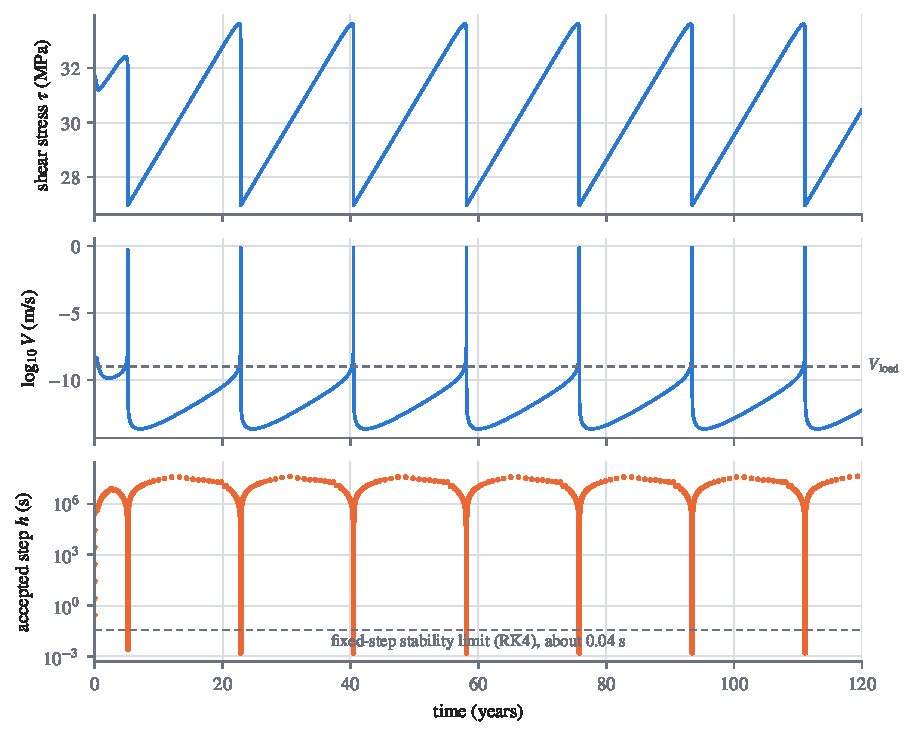
\includegraphics[width=0.88\textwidth]{slider_cycle}
\caption{Spring-block slider with $k=0.5\,k_{cr}$, integrated as the ODE system, Eq.~\eqref{eq:l3-ode}, with adaptive RK45 (relative tolerance $10^{-8}$). Top: shear stress; middle: slip rate on a logarithmic scale; bottom: size of every accepted time step (3\,782 steps in 120 yr). The step ranges from 1.7~ms during an event to 1.4~yr between events. The dashed line is a rough estimate of the largest stable step for a fixed-step RK4 scheme.}
\label{fig:l3-cycle}
\end{figure}

\subsection{Time integration: what the problem demands}

\paragraph{Time scales span ten orders of magnitude.} During an event the state variable relaxes at the rate $V/\Dc\sim80$~s$^{-1}$; between events the rate is $\Vl/\Dc=10^{-7}$~s$^{-1}$. A fixed time step must be small enough for the event and then be used for the 17.7 years in between. Using the stability bound of RK4 on the fastest rate gives $h\lesssim2.78/80\approx0.04$~s, so a fixed-step integration of one cycle would take about $1.5\times10^{10}$ steps. The adaptive integrator needs 538 steps per cycle: it takes steps of milliseconds during the event and steps of years in between (Figure~\ref{fig:l3-cycle}, bottom). This cost ratio is the argument for adaptive stepping.

\paragraph{The error tolerance controls accuracy, not stability.} Inside an event the smallest accepted step (1.7~ms) is about twenty times smaller than the stability limit just estimated. The step is therefore chosen by the accuracy requirement, and the problem is hard because it is rapidly varying, not because explicit integration is unstable. Whether to switch to an implicit method is decided by comparing these two limits; here no switch is needed.

\paragraph{Tolerance study.} Tightening the relative tolerance from $10^{-6}$ to $10^{-8}$ to $10^{-10}$ increases the number of steps in 120 yr from 1\,653 to 3\,782 to 9\,334, and changes the recurrence interval by less than $10^{-4}$~yr (17.65537, 17.65531, 17.65531). Cost grows slowly with accuracy, and a result that does not change under such a change in tolerance is converged in the sense that matters.

\subsection{Consistency checks}

\begin{enumerate}[itemsep=1pt,topsep=2pt]
\item \textbf{The first cycle is not representative.} In the reference run the first event slips 0.44~m and every later event slips 0.56~m, because the initial condition lies off the limit cycle. Results apply only once the solution is periodic: stress extrema, peak velocity and recurrence repeat to several digits.
\item \textbf{Slip balance.} Over a full cycle the spring stress returns to its starting value, so $\int\dot\tau\,\dd t=0$ and the slip per cycle equals $\Vl T_{rec}$. Here $10^{-9}\times17.655\times3.156\times10^{7}=0.557$~m, matching the integrated slip.
\item \textbf{Stress drop.} The drop in $\tau$ during an event must equal $k$ times the event slip. The computed drop is $33.62-26.96=6.67$~MPa; the slip it implies is $6.67/12.5=0.53$~m, close to the 0.56~m total (the small difference is the loading during the event).
\item \textbf{Peak velocity.} Radiation damping caps $V$ near (stress drop)/$\eta=6.67/5\approx1.3$~m/s. The computed peak, 0.77~m/s, is consistent in order of magnitude. A peak of $10^{3}$~m/s or $10^{-3}$~m/s would indicate an error in units or in $\eta$.
\item \textbf{Stiffness test.} The solution must change character at $k_{cr}$ (Table~\ref{tab:l3-kcr}). This is the cheapest test that the friction law, the aging law and the differentiated constraint have the correct signs.
\item \textbf{Constraint residual.} With $\tau$ carried as an extra state, $\tau-\tau_f-\eta V$ must stay at the integration tolerance (a few pascals at $10^{-8}$). A residual that is constant and non-zero from $t=0$ indicates an inconsistent initial condition; a residual that grows indicates a tolerance that is too loose.
\item \textbf{Tolerance test.} Repeating the run with the tolerance reduced by $10^2$ should leave event times and peak velocity unchanged in the reported digits.
\end{enumerate}

%======================================================================
\section{Frictional Heating and Heat Diffusion Away from the Fault}
\label{sec:l3-heat}
%======================================================================

\subsection{Heat source and governing equation}

The rate at which friction produces heat per unit fault area is
\begin{equation}
q(t)=\tau(t)\,V(t)\qquad[\text{W/m}^2].
\label{eq:l3-heat-rate}
\end{equation}
This is the quantity that connects Section~\ref{sec:l3-slider} to the present one: the slider provides $\tau(t)$ and $V(t)$, and the rock on either side of the fault must absorb $q$. In the limit of an infinitely thin slipping zone the heat is released at the plane $y=0$, where $y$ is the distance perpendicular to the fault, and spreads symmetrically, so each side receives $q_0=q/2$. Away from the fault the temperature rise $T(y,t)$ satisfies the diffusion equation
\begin{equation}
\frac{\partial T}{\partial t}=\alpha\,\frac{\partial^2T}{\partial y^2},\qquad y>0,
\label{eq:l3-diffusion}
\end{equation}
where $\alpha=k_{th}/(\rho c)$ is the thermal diffusivity, $k_{th}$ the thermal conductivity and $\rho c$ the volumetric heat capacity. We use $\alpha=10^{-6}$~m$^2$/s, $k_{th}=2.7$~W/(m\,K) and $\rho c=2.7\times10^6$~J/(m$^3$K) throughout. The fault enters the problem only through the boundary condition (Fourier's law),
\begin{equation}
-k_{th}\,\frac{\partial T}{\partial y}\Big|_{y=0}=q_0(t),\qquad T\to0\ \text{as } y\to\infty,
\label{eq:l3-bc}
\end{equation}
that is, a prescribed flux at $y=0$ and a fixed temperature far away. The pairing of a Neumann (flux) condition at the active boundary and a Dirichlet (value) condition at the inert one is typical of geophysical diffusion problems.

\begin{remark}[The same equation governs pore pressure]
Pore pressure $p(y,t)$ obeys $\partial p/\partial t=\alpha_{hy}\,\partial^2p/\partial y^2$ with a hydraulic diffusivity $\alpha_{hy}$, plus a coupling term in which rising temperature raises pressure. In a later lecture, pressure reduces the effective normal stress $\sigma$ in Eq.~\eqref{eq:l3-rsf}, which feeds back on $\tau$ and hence on $q$. A single tested diffusion solver will be used for both fields.
\end{remark}

\subsection{Scales before any grid is chosen}

The only length that the diffusion equation contains is the diffusion length $\delta(t)=\sqrt{\alpha t}$, the distance heat has spread by time $t$. With $\alpha=10^{-6}$~m$^2$/s:
\begin{center}
\small
\begin{tabular}{lcccc}
\toprule
elapsed time $t$ & 1 ms & 1 s & 12 s (one event) & 17.7 yr (one cycle) \\
\midrule
$\sqrt{\alpha t}$ & 30~$\mu$m & 1~mm & 3.5~mm & 24~m \\
\bottomrule
\end{tabular}
\end{center}
Two consequences shape every numerical decision later. First, the heated layer during an earthquake is millimetres thick, so the grid must resolve millimetres, not metres. Second, $\delta$ starts at zero and grows with time, so a grid fine enough at $t=1$~s may be too coarse at $t=1$~ms (Section~\ref{sec:l3-fd-verify}). Over the interseismic interval the heat spreads to tens of metres, a range of nearly four orders of magnitude in length scale; only the event and its aftermath are modeled here.

\subsection{How much heat, and how hot?}

Integrating $\tau V$ over one simulated event (the interval with $V>1$~mm/s, duration 12~s, slip 0.43~m, mean stress 29.7~MPa) gives a total of $Q=1.3\times10^{7}$~J/m$^2$, and the peak heating rate is $q_{max}=2.4\times10^{7}$~W/m$^2$.

A hand estimate of the temperature precedes any computation. For a constant flux $q_0$ switched on at $t=0$, the half-space solution is known in closed form,
\begin{equation}
T(y,t)=\frac{q_0}{k_{th}}\left[2\sqrt{\frac{\alpha t}{\pi}}\;e^{-y^2/4\alpha t}-y\,\mathrm{erfc}\!\left(\frac{y}{2\sqrt{\alpha t}}\right)\right],\qquad T(0,t)=\frac{2q_0}{k_{th}}\sqrt{\frac{\alpha t}{\pi}}.
\label{eq:l3-exact}
\end{equation}
Spread the event's heat uniformly over its duration: $q_0=Q/(2\times12\ \text{s})=5.3\times10^5$~W/m$^2$, so
\[
T(0,12\ \text{s})\approx\frac{2(5.3\times10^5)}{2.7}\sqrt{\frac{10^{-6}\times12}{\pi}}\approx 8\times10^{2}\ \text{K}.
\]
The full calculation with the actual $q(t)$, using the superposition integral for a time-varying flux,
\begin{equation}
T(0,t)=\frac{1}{k_{th}}\sqrt{\frac{\alpha}{\pi}}\int_0^t q_0(t')\,(t-t')^{-1/2}\,\dd t',
\end{equation}
gives a peak of about $2.3\times10^3$~K, reached about 10~s after the onset. The hand estimate is low by a factor of three because the heat is released mostly near the end of the event, and late heat has had less time to diffuse away. The sign of this bias is predictable, which makes the estimate a useful check.

Either number is unphysically large: it is above the melting temperature of rock. The reason is the assumption of a vanishing shear-zone thickness; real shear zones have finite width, and in the full model the fluid pressurization lowers $\tau$ as the fault heats, which reduces $q$. This feedback is exactly what the coupled model of later lectures will capture, and it is why temperature is a quantity that must be computed accurately and not guessed.

\begin{figure}[ht]
\centering
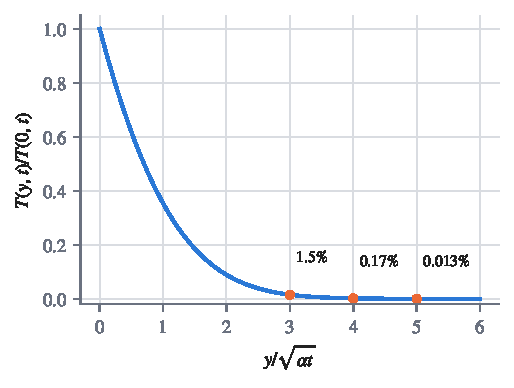
\includegraphics[width=0.52\textwidth]{heat_profile}
\caption{The constant-flux solution, Eq.~\eqref{eq:l3-exact}, normalized by its value at the fault, as a function of $y/\sqrt{\alpha t}$. The curve is universal: it has the same shape at all times, with only the length scale $\sqrt{\alpha t}$ changing. The temperature at $3\sqrt{\alpha t}$ is 1.5\% of the value at the fault, at $4\sqrt{\alpha t}$ it is 0.17\%, and at $5\sqrt{\alpha t}$ it is 0.013\%.}
\label{fig:l3-heat-profile}
\end{figure}

\subsection{The numerical problem}

The required quantity is $T(y,t)$, driven by a flux $q_0(t)$ that varies over many orders of magnitude and is itself produced by the slider. Discretizing only $y$ and keeping $t$ continuous turns Eq.~\eqref{eq:l3-diffusion} into a large system of ODEs, one per grid point, of the type treated in Section~\ref{sec:l3-slider} for two unknowns. This view (the method of lines) is used twice below: it explains the stability limit, and it determines how the diffusion solver is coupled to the slider.

%======================================================================
\section{Finite Differences for the Diffusion Equation}
\label{sec:l3-fd}
%======================================================================

\subsection{Structure of the analysis}

A finite-difference calculation is assessed by four questions, each with a failure mode that produces no error message.

\begin{enumerate}[itemsep=1pt,topsep=2pt]
\item \textbf{Is the discrete equation an approximation to the right equation, and of what order?} This is settled by a Taylor expansion (Sections~\ref{sec:l3-fd-space} and \ref{sec:l3-fd-time}).
\item \textbf{Is it stable?} An approximation can be accurate at every step and still blow up. A single dimensionless number decides (Section~\ref{sec:l3-fd-stab}).
\item \textbf{Are the boundary conditions as accurate as the interior, and do they conserve what should be conserved?} Boundaries are where order and energy are lost, and the loss is invisible on a plot (Section~\ref{sec:l3-fd-bc}).
\item \textbf{Is the complete implementation correct?} The tests are comparison with an exact solution, the rate at which the error falls under refinement, and a conserved quantity (Section~\ref{sec:l3-fd-verify}).
\end{enumerate}

For each of the four, the sections below give the criterion for a pass and the signature of a failure.

\subsection{Approximating derivatives on a grid}
\label{sec:l3-fd-space}

\begin{figure}[ht]
\centering
\begin{tikzpicture}[>=Stealth]
\def\dy{1.2}   % grid spacing in cm; nodes y_j = j*\dy, j = 0..9
% rock (y>0), mirror half-space (y<0), fault, far boundary
\fill[blue!6] (0,0) rectangle (10.8,2.4);
\draw[gray,dashed] (-1.8,0) rectangle (0,2.4);
\node[gray,font=\scriptsize,align=center] at (-0.9,1.2) {mirror image\\(no separate\\unknowns)};
\draw[orange!85!black,line width=2pt] (0,-0.05) -- (0,2.45);
\node[orange!85!black,font=\small,anchor=south] at (0,2.5) {fault, $y=0$};
\draw[line width=1.2pt] (10.8,0) -- (10.8,2.4);
\node[font=\small,anchor=west,align=left] at (10.95,1.2) {far boundary\\$T=0$};
% heat flux into the half-space
\draw[->,thick,orange!85!black] (0.05,0.3) -- (0.8,0.3);
\draw[->,thick,orange!85!black] (0.05,0.7) -- (0.8,0.7);
\node[orange!85!black,font=\scriptsize,anchor=west] at (0.08,1.0) {$q_0=q/2$};
% temperature profile (constant-flux solution) and its values at the nodes
\draw[thick,blue!70!black] plot[smooth] coordinates {(0.00,2.00) (0.60,1.55) (1.20,1.17) (1.80,0.86) (2.40,0.62) (3.00,0.43) (3.60,0.29) (4.20,0.19) (4.80,0.12) (5.40,0.08) (6.00,0.05) (6.60,0.03) (7.20,0.02) (7.80,0.01) (8.40,0.00) (9.00,0.00) (9.60,0.00) (10.20,0.00) (10.80,0.00)};
\foreach \j/\h in {0/2.00, 1/1.17, 2/0.62, 3/0.29, 4/0.12, 5/0.05, 6/0.02, 7/0.00, 8/0.00, 9/0.00} {
  \draw[gray,dotted] (\j*\dy,0) -- (\j*\dy,\h);
  \fill[blue!70!black] (\j*\dy,\h) circle (1.6pt);
  \fill (\j*\dy,0) circle (2pt);
}
\node[blue!70!black,font=\scriptsize,anchor=south west] at (4.85,0.12) {$T_j^n$};
% node axis and labels
\draw[->] (-1.8,0) -- (13.2,0) node[right,font=\small] {$y$};
\draw[fill=white] (-1.2,0) circle (2pt);
\node[gray,font=\scriptsize,anchor=north] at (-1.2,-0.62) {ghost node};
\foreach \x/\l in {-1.2/y_{-1}, 0/y_0, 1.2/y_1, 2.4/y_2, 3.6/\cdots, 4.8/y_{j-1},
                   6/y_j, 7.2/y_{j+1}, 8.4/\cdots, 9.6/\cdots, 10.8/y_N}
  \node[below,font=\small] at (\x,-0.08) {$\l$};
\draw[decorate,decoration={brace,amplitude=3pt,mirror}] (0,-0.95) -- (1.2,-0.95)
  node[midway,below=3pt,font=\scriptsize] {$\Delta y$};
\draw[decorate,decoration={brace,amplitude=3pt,mirror}] (6,-0.95) -- (7.2,-0.95)
  node[midway,below=3pt,font=\scriptsize] {$\Delta y$};
% diffusion length and domain size
\draw[<->] (0,2.95) -- (2.16,2.95) node[midway,above,font=\scriptsize] {$\sqrt{\alpha t}$};
\draw[<->] (0,3.65) -- (10.8,3.65)
  node[midway,above,font=\scriptsize] {$y_N\gtrsim5\sqrt{\alpha\,t_{final}}$};
\draw[dotted,gray] (2.16,2.4) -- (2.16,3.0);
\draw[dotted,gray] (10.8,2.4) -- (10.8,3.7);
\end{tikzpicture}
\caption{Spatial discretization next to the fault. Frictional heat generated on the plane $y=0$ enters the half-space $y\ge0$ at $q_0=q/2$ per side. The temperature $T_j^n$ is stored at the nodes $y_j=j\,\Delta y$, $j=0,\dots,N$, and $T=0$ is imposed at the far boundary $y_N$. The node $y_{-1}$ is a fictitious ghost value used for the flux condition (Section~\ref{sec:l3-fd-bc}). The heated layer has a thickness of order $\sqrt{\alpha t}$, so $y_N$ must exceed several multiples of $\sqrt{\alpha t_{final}}$. The profile shown is the constant-flux solution, Eq.~\eqref{eq:l3-exact}.}
\label{fig:l3-grid}
\end{figure}

Replace the half-line $y\ge0$ by points $y_j=j\,\Delta y$, $j=0,\dots,N$, with $y_0=0$ at the fault and $y_N$ the far boundary. Let $T_j^n\approx T(y_j,t^n)$ with $t^n=n\,\Delta t$. To approximate $\partial^2T/\partial y^2$ at an interior point, expand the neighbors in Taylor series about $y_j$ at fixed time:
\begin{align}
T_{j+1}&=T_j+\Delta y\,T_j'+\tfrac12\Delta y^2T_j''+\tfrac16\Delta y^3T_j'''+\tfrac1{24}\Delta y^4T_j''''+\order{\Delta y^5},\\
T_{j-1}&=T_j-\Delta y\,T_j'+\tfrac12\Delta y^2T_j''-\tfrac16\Delta y^3T_j'''+\tfrac1{24}\Delta y^4T_j''''+\order{\Delta y^5}.
\end{align}
where primes denote $\partial/\partial y$ evaluated at $y_j$, at fixed time (the time index is suppressed in this calculation).

Adding the two, the odd-order terms cancel exactly:
\begin{equation}
\frac{\partial^2T}{\partial y^2}\Big|_{y_j}=\frac{T_{j+1}-2T_j+T_{j-1}}{\Delta y^2}-\frac{\Delta y^2}{12}\,T_j''''+\order{\Delta y^4}.
\label{eq:l3-central}
\end{equation}
The first term on the right is the \textbf{central difference}. The leading truncation error is proportional to $\Delta y^2$: the scheme is second order in space, and its error is largest where the solution has sharp fine-scale structure ($T''''$ large), such as the first few $\sqrt{\alpha t}$ at early times.

The cancellation depends on $y_j$ sitting exactly midway between its neighbors. A first derivative from a one-sided difference does not enjoy it:
\begin{equation}
\frac{\partial T}{\partial y}\Big|_{y_j}=\frac{T_{j+1}-T_j}{\Delta y}+\order{\Delta y},\qquad
\frac{\partial T}{\partial y}\Big|_{y_j}=\frac{T_{j+1}-T_{j-1}}{2\Delta y}+\order{\Delta y^2}.
\label{eq:l3-first}
\end{equation}
The one-sided formula is first order and the centered one is second order, at the same cost. This matters at the fault, where one neighbor is missing (Section~\ref{sec:l3-fd-bc}).

\subsection{Marching in time: the explicit scheme}
\label{sec:l3-fd-time}

The explicit scheme applies forward Euler in time, as in the earlier ODE lectures, at each grid point, together with the central difference in space. Write the diffusion equation, Eq.~\eqref{eq:l3-diffusion}, at the node $(y_j,t^n)$:
\begin{equation}
\frac{\partial T}{\partial t}\bigg|_j^n=\alpha\,\frac{\partial^2T}{\partial y^2}\bigg|_j^n.
\end{equation}
For the time derivative, expand $T$ forward in time about $t^n$ at fixed $y_j$:
\begin{equation}
T_j^{n+1}=T_j^n+\Delta t\,\frac{\partial T}{\partial t}\bigg|_j^n+\frac{\Delta t^2}{2}\frac{\partial^2T}{\partial t^2}\bigg|_j^n+\order{\Delta t^3},
\end{equation}
which gives
\begin{equation}
\frac{\partial T}{\partial t}\bigg|_j^n=\frac{T_j^{n+1}-T_j^n}{\Delta t}-\frac{\Delta t}{2}\frac{\partial^2T}{\partial t^2}\bigg|_j^n+\order{\Delta t^2}.
\end{equation}
For the space derivative, use Eq.~\eqref{eq:l3-central} at time level $n$:
\begin{equation}
\frac{\partial^2T}{\partial y^2}\bigg|_j^n=\frac{T_{j+1}^n-2T_j^n+T_{j-1}^n}{\Delta y^2}-\frac{\Delta y^2}{12}\frac{\partial^4T}{\partial y^4}\bigg|_j^n+\order{\Delta y^4}.
\end{equation}
Substituting both into the diffusion equation and collecting the terms that contain higher derivatives on the right-hand side,
\begin{equation}
\frac{T_j^{n+1}-T_j^n}{\Delta t}=\alpha\,\frac{T_{j+1}^n-2T_j^n+T_{j-1}^n}{\Delta y^2}+\underbrace{\frac{\Delta t}{2}\frac{\partial^2T}{\partial t^2}-\alpha\frac{\Delta y^2}{12}\frac{\partial^4T}{\partial y^4}}_{\text{truncation error}\;=\;\order{\Delta t}+\order{\Delta y^2}}.
\end{equation}
The scheme is obtained by dropping the truncation error. The result contains a single unknown, $T_j^{n+1}$, because every other quantity is evaluated at time level $n$. Multiplying by $\Delta t$ and solving for $T_j^{n+1}$ gives the FTCS (forward-time, centered-space) update
\begin{equation}
T_j^{n+1}=T_j^n+s\,\big(T_{j+1}^n-2T_j^n+T_{j-1}^n\big),\qquad s\equiv\frac{\alpha\,\Delta t}{\Delta y^2},
\label{eq:l3-ftcs}
\end{equation}
where $s$ is the only combination of $\alpha$, $\Delta t$ and $\Delta y$ that enters the update.

The dimensionless \textbf{diffusion number} $s$ is the most important quantity in the scheme. Equation~\eqref{eq:l3-ftcs} can be rewritten as $T_j^{n+1}=(1-2s)T_j^n+sT_{j+1}^n+sT_{j-1}^n$, a weighted average with weights summing to one. For $s\le\tfrac12$ all weights are non-negative, so each new value lies between the smallest and largest of the three old values and the scheme cannot create new extrema, which is the correct behavior of diffusion. For $s>\tfrac12$ the middle weight is negative, and the average interpretation is lost.

\begin{figure}[ht]
\centering
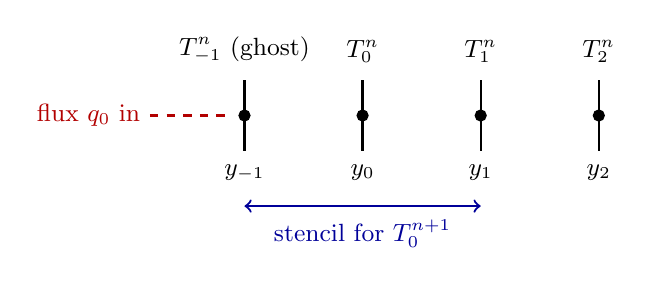
\begin{tikzpicture}[scale=1.0]
\def\dy{1.5}
\foreach \j/\lab in {-1/{-1}, 0/{0}, 1/{1}, 2/{2}} {
  \draw[thick] (\j*\dy,0) -- (\j*\dy,0.9);
  \filldraw[black] (\j*\dy,0.45) circle (2pt);
  \node[below] at (\j*\dy,-0.05) {\small $y_{\lab}$};
}
\node[above] at (-\dy,1.0) {\small $T_{-1}^n$ (ghost)};
\node[above] at (0,1.0) {\small $T_0^n$};
\node[above] at (\dy,1.0) {\small $T_1^n$};
\node[above] at (2*\dy,1.0) {\small $T_2^n$};
\draw[<->,thick,blue!60!black] (-\dy,-0.7) -- (\dy,-0.7);
\node[below,blue!60!black] at (0,-0.75) {\small stencil for $T_0^{n+1}$};
\draw[dashed,red!70!black,thick] (-1.8*\dy,0.45) -- (-\dy-0.15,0.45);
\node[left,red!70!black] at (-1.8*\dy,0.45) {\small flux $q_0$ in};
\end{tikzpicture}
\caption{The explicit stencil. The update at node $j$ uses the old values at $j-1$, $j$, $j+1$ and nothing from the new time level. At the fault ($j=0$) the node $j=-1$ does not exist physically, so a ghost value is constructed from the flux condition (Section~\ref{sec:l3-fd-bc}).}
\label{fig:l3-stencil}
\end{figure}

\subsection{Stability}
\label{sec:l3-fd-stab}

The truncation errors above are $\order{\Delta t}+\order{\Delta y^2}$, so FTCS is consistent. Consistency is not sufficient: forward Euler on $\dot y=\lambda y$ is consistent for every $h$ yet unstable unless $|1+h\lambda|\le1$, i.e.\ $h\le2/|\lambda|$ for real negative $\lambda$. The same applies here, and there are two independent ways to see what $s$ must satisfy.

\paragraph{Fourier (von Neumann) analysis.} Insert a single wave $T_j^n=\xi^n e^{\mathrm{i}\theta j}$, where $\theta=k\Delta y\in[-\pi,\pi]$ is the phase advance per cell, into Eq.~\eqref{eq:l3-ftcs}. The per-step amplification factor of the wave is
\begin{equation}
\xi(\theta)=1-4s\sin^2\!\frac{\theta}{2}\in[1-4s,\,1].
\label{eq:l3-vn}
\end{equation}
Stability needs $|\xi|\le1$ for every representable wave. The dangerous one is the checkerboard $\theta=\pi$ (alternating sign from node to node), for which $\xi=1-4s$; requiring $|1-4s|\le1$ gives
\begin{equation}
\boxed{\,s\le\tfrac12\quad\Longleftrightarrow\quad\Delta t\le\frac{\Delta y^2}{2\alpha}\,}.
\label{eq:l3-bound}
\end{equation}

\paragraph{Method of lines.} Discretizing only in space leaves the time derivative continuous. With $T_0=T_N=0$ imposed (homogeneous Dirichlet conditions, for this illustration) the interior values $T_1,\dots,T_{N-1}$ obey
\begin{equation}
\frac{\dd T_j}{\dd t}=\frac{\alpha}{\Delta y^2}\big(T_{j+1}-2T_j+T_{j-1}\big),\qquad j=1,\dots,N-1,
\end{equation}
which is a linear ODE system. Written out as a vector equation,
\begin{equation}
\frac{\dd}{\dd t}
\begin{pmatrix}T_1\\T_2\\T_3\\\vdots\\T_{N-2}\\T_{N-1}\end{pmatrix}
=\frac{\alpha}{\Delta y^2}
\begin{pmatrix}
-2 & 1 & & & & \\
1 & -2 & 1 & & & \\
 & 1 & -2 & 1 & & \\
 & & \ddots & \ddots & \ddots & \\
 & & & 1 & -2 & 1\\
 & & & & 1 & -2
\end{pmatrix}
\begin{pmatrix}T_1\\T_2\\T_3\\\vdots\\T_{N-2}\\T_{N-1}\end{pmatrix},
\qquad\text{i.e.}\qquad
\dot{\mathbf T}=\frac{\alpha}{\Delta y^2}\,D\,\mathbf T,
\end{equation}
where $D$ is the $(N-1)\times(N-1)$ tridiagonal matrix with $-2$ on the diagonal and $1$ on the two adjacent diagonals; empty entries are zero. The matrix $\alpha D/\Delta y^2$ plays the role of the Jacobian in the ODE lectures. Its eigenvalues are known in closed form,
\begin{equation}
\lambda_k=-\frac{4\alpha}{\Delta y^2}\sin^2\!\frac{k\pi}{2N},\qquad k=1,\dots,N-1,
\end{equation}
all real and negative. The most negative one tends to $\lambda_{max}\to-4\alpha/\Delta y^2$ as the grid is refined. Applying forward Euler to this system gives
\begin{equation}
\mathbf T^{n+1}=\mathbf T^n+\Delta t\,\frac{\alpha}{\Delta y^2}\,D\,\mathbf T^n=(I+s\,D)\,\mathbf T^n,
\end{equation}
which is Eq.~\eqref{eq:l3-ftcs} written for all nodes at once. The eigenvalues of $I+sD$ are $1+s\,\mu_k$, with $\mu_k=-4\sin^2(k\pi/2N)\in(-4,0)$, and forward Euler is stable if all of them lie in $[-1,1]$. The most restrictive is $k=N-1$, where $\mu_k\to-4$, so the condition is $|1-4s|\le1$, i.e.\ $\Delta t\le2/|\lambda_{max}|=\Delta y^2/(2\alpha)$. This is the same bound as above, obtained without Fourier analysis, and the agreement of the two derivations is itself a check on the algebra.

This means that refining the grid makes the ODE system stiffer, with a rate that grows as $1/\Delta y^2$. For $\alpha=10^{-6}$~m$^2$/s: $\Delta y=0.1$~mm requires $\Delta t\le5$~ms; $\Delta y=10$~$\mu$m requires $\Delta t\le50$~$\mu$s. Resolution is paid for twice, once in the number of nodes and once in the number of steps.

\begin{figure}[ht]
\centering
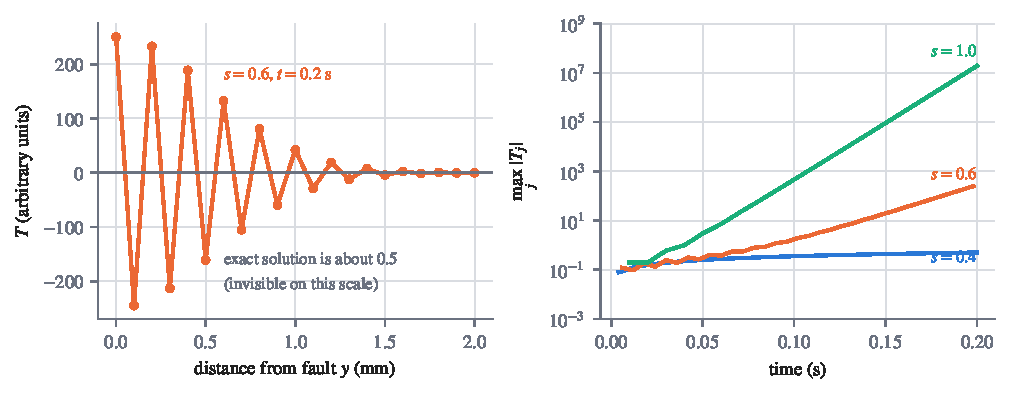
\includegraphics[width=0.96\textwidth]{fd_instability}
\caption{Violating $s\le1/2$ ($\Delta y=0.1$~mm, $\alpha=1$~mm$^2$/s, unit flux gradient). Left: profile near the fault at $t=0.2$~s for $s=0.6$; the solution alternates in sign from node to node with amplitude of order 250, whereas the exact value is about 0.5. Right: the largest absolute value of $T$ over the grid as a function of time; for $s=0.4$ it is stable and for $s=0.6$ and $s=1$ it grows geometrically.}
\label{fig:l3-instability}
\end{figure}

\paragraph{Appearance of the instability.} An unstable run does not stop with an error message; it produces a checkerboard whose amplitude grows by $|1-4s|$ at every step (Figure~\ref{fig:l3-instability}). A mild violation is more dangerous than a gross one, because it can look correct for a long time. With $\Delta y=0.1$~mm and $\alpha=1$~mm$^2$/s, the temperature at the fault for $s=0.51$ is $0.518$ at $t=0.2$~s against an exact $0.505$ (a 3\% error that could be taken for discretization error), then $-2.0$ at $t=1$~s, $-4.8\times10^3$ at $t=2$~s and $-1.6\times10^{10}$ at $t=4$~s. At $s=0.5$ the result remains accurate at all these times. The value of $s$ should therefore be checked explicitly; a variable time step is the usual way an $s$ slightly above one-half goes unnoticed.

\paragraph{Consistency plus stability gives convergence.} The Lax equivalence theorem states that, for a well-posed linear problem, a consistent and stable scheme converges as the grid is refined, and that a scheme which converges must be both. This is why checking the order of the truncation error and checking $s\le\frac12$ are the two halves of one guarantee, and why a convergence study (Section~\ref{sec:l3-fd-verify}) can be trusted only after stability has been established.

\subsection{Boundary conditions}
\label{sec:l3-fd-bc}

\paragraph{Far boundary.} At $y_N$ we impose $T=0$. This is correct only as long as no appreciable heat has reached it. The solution at $y=c\sqrt{\alpha t}$ relative to the fault value is 1.5\%, 0.17\% and 0.013\% for $c=3,4,5$ (Figure~\ref{fig:l3-heat-profile}), so a conservative rule is
\begin{equation}
y_N\gtrsim5\sqrt{\alpha\,t_{final}},
\label{eq:l3-domain}
\end{equation}
re-checked whenever the simulated time changes.

\paragraph{Fault boundary.} The condition $-k_{th}\,\partial_yT=q_0$ involves a derivative, and the update at $j=0$ needs $T_{-1}$, which does not exist. A \textbf{ghost point} is a fictitious value chosen so that the centered difference of Eq.~\eqref{eq:l3-first} at $j=0$ reproduces the boundary condition. The flux enters the rock, so the temperature decreases away from the fault, $\partial_yT|_0=-q_0/k_{th}$, and
\begin{equation}
\frac{T_1^n-T_{-1}^n}{2\Delta y}=-\frac{q_0}{k_{th}}\;\;\Longrightarrow\;\;T_{-1}^n=T_1^n+\frac{2\Delta y\,q_0}{k_{th}}.
\end{equation}
Substituting into Eq.~\eqref{eq:l3-ftcs} at $j=0$,
\begin{equation}
T_0^{n+1}=T_0^n+2s\,(T_1^n-T_0^n)+\frac{2s\,\Delta y\,q_0(t^n)}{k_{th}}.
\label{eq:l3-bc-update}
\end{equation}
There is a physical reading of the two factors of 2. Node 0 owns only the half-cell of width $\Delta y/2$ next to the boundary. Heat balance on it reads $(\Delta y/2)\,\dot T_0=\alpha(T_1-T_0)/\Delta y+\alpha q_0/k_{th}$, and multiplying by $\Delta t$ gives Eq.~\eqref{eq:l3-bc-update} exactly. This control-volume view is how the same condition is derived in the finite-volume method, and it shows what goes wrong if the factors are dropped.

\paragraph{Errors in the boundary treatment.} Each of the following gives a stable, smooth-looking solution at $\Delta y=0.1$~mm, $\alpha=1$~mm$^2$/s, $t=1$~s with unit flux gradient. The exact value is $T(0)=1.1284$ and the exact heat content $\int T\,\dd y=\alpha t\,q_0/k_{th}=1$.

\begin{center}
\small
\begin{tabular}{lccc}
\toprule
boundary treatment & $T(0)$ & heat content & error decays as \\
\midrule
ghost point, Eq.~\eqref{eq:l3-bc-update} & 1.1277 & 1.000 & $\Delta y^2$ \\
node treated as a full cell (factors 2 dropped) & 1.0791 & 0.946 & $\Delta y$ \\
one-sided gradient $T_0=T_1+\Delta y\,q_0/k_{th}$ & 1.1790 & 1.059 & $\Delta y$ \\
sign of the flux reversed & $-1.1277$ & $-1.000$ & (obvious) \\
\bottomrule
\end{tabular}
\end{center}
The reversed sign shows itself in the first plot. The other two errors are about 5\% and look like ordinary discretization error; they reveal themselves only through the convergence rate (the error falls by a factor of 2, not 4, when $\Delta y$ is halved) and through the heat balance (Figure~\ref{fig:l3-convergence}). A related mistake, forgetting that the flux splits into two sides ($q_0=q/2$), multiplies every temperature by exactly 2 and can be caught only by comparing the heat in the rock with $\tfrac12\int\tau V\,\dd t$.

\subsection{Preview: implicit time stepping}

The bound $\Delta t\le\Delta y^2/(2\alpha)$ is expensive when coupled to the slider. With $\Delta y=0.1$~mm, covering a single 17.7~yr interseismic interval with 5~ms steps takes about $10^{11}$ steps, although the slider itself needs only a few hundred. Evaluating the spatial difference at the new time level,
\begin{equation}
\frac{T_j^{n+1}-T_j^n}{\Delta t}=\alpha\,\frac{T_{j+1}^{n+1}-2T_j^{n+1}+T_{j-1}^{n+1}}{\Delta y^2},
\end{equation}
gives BTCS, with $\xi(\theta)=1/\big(1+4s\sin^2(\theta/2)\big)\in(0,1]$ for every $s>0$ and thus no stability limit on $\Delta t$. The price is a tridiagonal linear system at each step, which is cheap. This is the backward Euler method from the ODE lectures applied to the stiff system above. The coupled calculation in a later lecture will make this switch, and the stability analysis here is the justification for it.

\subsection{Verification}
\label{sec:l3-fd-verify}

Visual plausibility of a profile is not a test. Four checks are used, each with a numerical outcome. The benchmark throughout is Eq.~\eqref{eq:l3-exact}, computed in units of mm and seconds with $\alpha=1$~mm$^2$/s and $q_0/k_{th}=1$~K/mm, so $T(0,t)=2\sqrt{t/\pi}$ and $T(0,1\ \text{s})=1.1284$~K.

\paragraph{1. Compare with the exact solution.} Equation~\eqref{eq:l3-exact} is the only closed-form solution needed. An implementation that does not reproduce it for a constant flux cannot be relied on for a variable flux.

\paragraph{2. Refine and read the rate.} Reduce $\Delta y$ by 2 at a time step small enough that time error is negligible; the error in $T(0)$ at $t=1$~s should fall by a factor of 4.

\begin{center}
\small
\begin{tabular}{lcccc}
\toprule
$\Delta y$ (mm) & 0.4 & 0.2 & 0.1 & 0.05 \\
\midrule
error in $T(0)$ & $1.15\times10^{-2}$ & $2.83\times10^{-3}$ & $7.04\times10^{-4}$ & $1.75\times10^{-4}$ \\
ratio to previous & --- & 4.05 & 4.02 & 4.03 \\
\bottomrule
\end{tabular}
\end{center}
In time, at fixed $\Delta y=0.1$~mm, halving $\Delta t$ halves the error (ratios 2.01, 2.01, 2.02, forward Euler is first order). If $s$ is kept fixed at 0.25, then $\Delta t\propto\Delta y^2$ and the combined error falls by a factor of 4.00 per halving of $\Delta y$. The scheme behaves as second order in $\Delta y$ along any path of constant $s$, which is how it is used in practice. An error that falls by a factor of 2 where 4 is expected indicates that a boundary or another lower-order component limits the accuracy (Figure~\ref{fig:l3-convergence}).

\begin{figure}[ht]
\centering
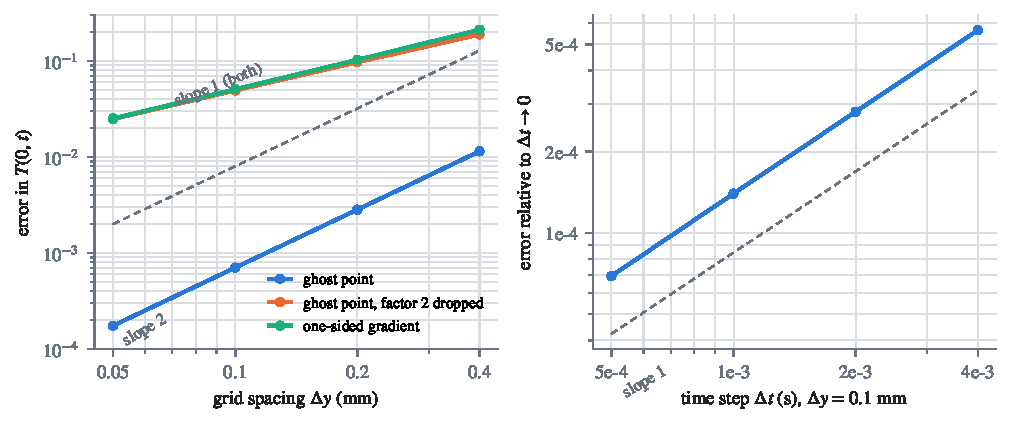
\includegraphics[width=0.96\textwidth]{fd_convergence}
\caption{Left: error in the fault temperature at $t=1$~s against grid spacing for the ghost-point boundary and for the two lower-order treatments of the previous table. Right: error against time step at $\Delta y=0.1$~mm, relative to the limit $\Delta t\to0$. The ghost-point treatment follows a slope of 2; the other two have slope 1 and lose a factor of about 70 in accuracy at $\Delta y=0.1$~mm.}
\label{fig:l3-convergence}
\end{figure}

\paragraph{3. Check a conserved quantity.} The heat content $\int T\,\dd y$ must equal $\alpha\,t\,q_0/k_{th}$, independent of the detailed profile. It is a one-line check, it catches errors in the boundary, and the table above shows it reading 0.946 and 1.059 for the two faulty closures. Two cautions. The integral must be evaluated with the trapezoid rule (half weight at the boundary node), because the correct scheme itself gives 1.056 with a plain sum; the checking tool can be wrong too. And when the calculation is coupled to the slider, the heat in the rock must equal $\tfrac12\int\tau V\,\dd t$.

\paragraph{4. Check the domain and the early times.} For a unit flux, with $\Delta y=0.1$~mm, $\Delta t=10^{-3}$~s, the error in $T(0)$ is $5\times10^{-5}$ times the exact value when the domain is $3.2\sqrt{\alpha t}$ long ($t=10$~s, $L=10$~mm), 2.2\% for $1.6\sqrt{\alpha t}$ and 20\% for $0.9\sqrt{\alpha t}$. A domain that is too short does not generate any artefact visible in the interior; it simply lowers the temperature through the Dirichlet condition. The grid can also be too coarse for early times: for $\Delta y=0.1$~mm the relative error in $T(0)$ is 49\% at $t=1$~ms ($\sqrt{\alpha t}/\Delta y=0.3$), 7.2\% at 10~ms (1.0), 0.62\% at 0.1~s (3.2) and 0.061\% at 1~s (10). A good working rule is $\sqrt{\alpha t}\gtrsim3\,\Delta y$; at earlier times the numerical solution is only qualitatively right. The same grid can therefore pass a refinement test at 1~s and fail one at 1~ms.

\subsection{Symptoms and likely causes}

\begin{center}
\small
\renewcommand{\arraystretch}{1.15}
\begin{tabular}{p{0.38\textwidth}p{0.55\textwidth}}
\toprule
Symptom & Likely cause \\
\midrule
Alternating signs between nodes, amplitude growing & $s>\tfrac12$, Eq.~\eqref{eq:l3-bound}; print $s$ at each step \\
Temperature negative where heat is being injected & sign of the flux in the ghost-point update \\
Smooth profile but error halves (not quarters) under refinement & boundary closure of low order; node treated as a full cell \\
Heat content differs from $\alpha t q_0/k_{th}$ by a few percent & boundary update; trapezoid weights in the check \\
Temperature exactly twice the expected value & flux not divided between the two sides \\
Temperature at the fault drops when the domain is shortened & domain shorter than $5\sqrt{\alpha t_{final}}$ \\
Early-time error large, late-time error small & grid coarse compared with $\sqrt{\alpha t}$ at early $t$ \\
Slider: first events differ from later ones & spin-up transient; discard until periodic \\
Slider: velocity cap far from (stress drop)/$\eta$ & units, $\eta$, or the term $\eta V$ missing from the denominator of Eq.~\eqref{eq:l3-ode} \\
Slider: cycles correct but $\tau$ offset by a constant & initial condition violating the constraint, Eq.~\eqref{eq:l3-constraint} \\
\bottomrule
\end{tabular}
\end{center}

%======================================================================
\section{Summary}
\label{sec:l3-summary}
%======================================================================

\begin{itemize}[itemsep=2pt,topsep=2pt]
\item The spring-block slider is two ODEs plus one algebraic constraint. Differentiating the constraint gives an ODE system in $(\ln V,\theta)$, which an adaptive Runge--Kutta method integrates with steps from milliseconds to years in one run. The initial condition must satisfy the constraint, and the constraint residual should be monitored. Check the slip balance, the stress drop, the peak velocity and the transition at $k_{cr}$.
\item Frictional heating $q=\tau V$ drives a diffusion problem with a flux boundary condition at the fault. The diffusion length $\sqrt{\alpha t}$ sets the grid, the domain and a hand estimate of the temperature, and the constant-flux solution is the benchmark.
\item The explicit finite-difference scheme is second order in space and first order in time. It is stable only if $s=\alpha\Delta t/\Delta y^2\le\tfrac12$, which can be derived in two ways that agree. The cost grows as $1/\Delta y^2$.
\item Boundary conditions are where silent errors enter. The ghost-point treatment is second order and conserves heat; two plausible alternatives are first order and look correct.
\item Verification means a benchmark, the observed convergence rate, a conservation check, and checks of the domain size and the early-time resolution.
\end{itemize}

%======================================================================
\section{Notation}
\label{sec:l3-notation}
%======================================================================

\begin{center}
\small
\begin{tabular}{ll}
\toprule
Symbol & Meaning \\
\midrule
$\tau$, $\tau_f$ & shear stress; frictional strength \\
$V$, $\Vl$ & slip rate; plate (loading) velocity \\
$\theta$, $\Dc$ & state variable; characteristic slip distance \\
$\sigma$ & effective normal stress \\
$a$, $b$, $\mu^*$, $V^*$ & rate-and-state parameters and reference values \\
$k$, $k_{cr}$ & spring stiffness; critical stiffness \\
$\eta=G/(2\beta)$ & radiation-damping coefficient \\
$x=\ln(V/V^*)$ & state variable replacing $V$ \\
$q=\tau V$, $q_0=q/2$ & frictional heating rate; flux into one side \\
$T(y,t)$ & temperature rise; $y$ is distance from the fault \\
$\alpha$, $k_{th}$, $\rho c$ & thermal diffusivity, conductivity, heat capacity \\
$\sqrt{\alpha t}$ & diffusion length \\
$\Delta y$, $\Delta t$, $T_j^n$ & grid spacing, time step, grid value \\
$s=\alpha\Delta t/\Delta y^2$ & diffusion number \\
$\xi(\theta)$ & amplification factor of a Fourier mode \\
\bottomrule
\end{tabular}
\end{center}

%======================================================================
\section{Suggested Reading}
\label{sec:l3-reading}
%======================================================================

\begin{itemize}[itemsep=2pt,topsep=2pt]
\item J.\,R.\ Rice and A.\,L.\ Ruina (1983), Stability of steady frictional slipping, \emph{J.\ Appl.\ Mech.}\ 50, 343--349. The linear stability analysis behind Eq.~\eqref{eq:l3-kcr}.
\item J.\,R.\ Rice (1993), Spatio-temporal complexity of slip on a fault, \emph{J.\ Geophys.\ Res.}\ 98, 9885--9907. The radiation-damping approximation and the aging-law slider.
\item H.\,S.\ Carslaw and J.\,C.\ Jaeger (1959), \emph{Conduction of Heat in Solids}, 2nd ed., Oxford University Press. The solution Eq.~\eqref{eq:l3-exact} and its relatives.
\item R.\,J.\ LeVeque (2007), \emph{Finite Difference Methods for Ordinary and Partial Differential Equations}, SIAM. Chapters on the heat equation, stability and boundary conditions.
\item J.\,R.\ Rice (2006), Heating and weakening of faults during earthquake slip, \emph{J.\ Geophys.\ Res.}\ 111, B05311. Where the temperature estimate of Section~\ref{sec:l3-heat} leads.
\end{itemize}

%======================================================================
\section{Practice Problems: Numerical Pitfalls}
\label{sec:l3-problems}
%======================================================================

\subsection*{Problem 1: initial transient in the slider}

Integration of the slider of Section~\ref{sec:l3-slider} gives a slip of 0.44~m in the first event and 0.56~m in all later events, with a recurrence interval of 17.655~yr. Determine whether this indicates an error.

\solution It does not. The initial condition ($\theta$ at half its steady-state value) lies off the limit cycle, and the first event occurs at 5.2~yr, before a full recurrence interval has elapsed, so the first cycle is a transient. The slip balance holds for the later events: $\Vl T_{rec}=10^{-9}\times17.655\times3.156\times10^7=0.557$~m. An actual error would appear as later events that differ from $\Vl T_{rec}$ or from one another.

\subsection*{Problem 2: the cost of a fixed step}

Estimate the number of steps a fixed-step RK4 integration needs for one cycle, using the largest slip rate $V_{max}=0.77$~m/s, $\Dc=10$~mm and the RK4 real-axis stability limit $|h\lambda|\le2.78$. Compare with the 538 steps taken by the adaptive integrator.

\solution The fastest rate is $\lambda\approx V_{max}/\Dc=77$~s$^{-1}$, so $h\le2.78/77=0.036$~s. One cycle is $5.57\times10^{8}$~s, giving $1.5\times10^{10}$ steps. The adaptive integrator takes $3\times10^{7}$ times fewer steps. The estimate is a lower bound on the fixed-step cost, since accuracy may require smaller steps than stability. The cost is set by the ratio of the fastest to the slowest time scale, which an adaptive integrator does not pay.

\subsection*{Problem 3: a time step that is slightly too large}

For $\Delta y=0.1$~mm and $\alpha=1$~mm$^2$/s, the explicit scheme is run with $\Delta t=5.1$~ms. At $t=0.2$~s the fault temperature is $0.518$, against an exact $0.505$, a 3\% error. Determine whether this error is a discretization error.

\solution It is not. Here $s=0.51>\tfrac12$. The checkerboard mode grows by $|1-4s|=1.04$ per step, which is not yet visible at 0.2~s (40 steps) but which has taken the fault temperature to $-2.0$ at $t=1$~s, $-4.8\times10^3$ at 2~s and $-1.6\times10^{10}$ at 4~s. At $s=0.5$ the same code is accurate at all four times. The 3\% error was the beginning of the instability, not a discretization error. The stable choice is $\Delta t\le\Delta y^2/(2\alpha)=5$~ms.

\subsection*{Problem 4: two boundary errors that look like accuracy limits}

At $\Delta y=0.1$~mm, one code gives $T(0)=1.079$ and heat content 0.946 at $t=1$~s; another gives $T(0)=1.179$ and heat content 1.059. The exact values are 1.128 and 1.000. Halving $\Delta y$ in each code gives $T(0)=1.104$ and $T(0)=1.154$ respectively. Identify the error in each and explain why neither is visible in a plot of the profile.

\solution Halving $\Delta y$ reduces the error from $4.9\times10^{-2}$ to $2.5\times10^{-2}$ in the first code and from $5.1\times10^{-2}$ to $2.5\times10^{-2}$ in the second: factors of 2, instead of the 4 that a second-order scheme gives. Both have a first-order boundary. In the first code the factors of 2 in Eq.~\eqref{eq:l3-bc-update} were dropped, so the boundary node is treated as a full cell and it holds too little heat (0.946). In the second the gradient was imposed with a one-sided difference, $T_0=T_1+\Delta y\,q_0/k_{th}$, which has an $\order{\Delta y}$ error and gives too much heat (1.059). Both profiles are smooth and about 5\% off, so a plot will not reveal either; the convergence rate and the heat content do.

\subsection*{Problem 5: domain and early times}

A simulation to $t_{final}=10$~s with $\alpha=1$~mm$^2$/s uses a domain of length $L=3$~mm and $\Delta y=0.1$~mm, and is repeated to $t=1$~ms to examine the onset of heating. At 10~s the fault temperature is 20\% low; at 1~ms it is 49\% low, although the 10~s run converges under refinement. Explain both discrepancies and choose $L$ and $\Delta y$ for both times.

\solution At 10~s, $\sqrt{\alpha t}=3.2$~mm, so $L=3$~mm is $0.9\sqrt{\alpha t}$: the Dirichlet condition removes heat that should still be in the rock. Eq.~\eqref{eq:l3-domain} gives $L\gtrsim16$~mm; $L=10$~mm ($3.2\sqrt{\alpha t}$) already reduces the error to $5\times10^{-5}$. At 1~ms the diffusion length is 0.032~mm, a third of the grid spacing, so the heated layer is less than one cell thick, and a refinement test at 10~s carries no information about it. An error below 1\% at 1~ms requires $\sqrt{\alpha t}\ge3\Delta y$, i.e.\ $\Delta y\le10$~$\mu$m, which requires $\Delta t\le\Delta y^2/(2\alpha)=50$~$\mu$s. A single uniform grid cannot serve both times economically, which motivates non-uniform grids and the finite-volume method.
 -----------------------------------------------------------------------
 
%\printbibliography

\end{document}
